
%% bare_jrnl_compsoc.tex
%% V1.4b
%% 2015/08/26
%% by Michael Shell
%% See:
%% http://www.michaelshell.org/
%% for current contact information.
%%
%% This is a skeleton file demonstrating the use of IEEEtran.cls
%% (requires IEEEtran.cls version 1.8b or later) with an IEEE
%% Computer Society journal paper.
%%
%% Support sites:
%% http://www.michaelshell.org/tex/ieeetran/
%% http://www.ctan.org/pkg/ieeetran
%% and
%% http://www.ieee.org/

%%*************************************************************************
%% Legal Notice:
%% This code is offered as-is without any warranty either expressed or
%% implied; without even the implied warranty of MERCHANTABILITY or
%% FITNESS FOR A PARTICULAR PURPOSE! 
%% User assumes all risk.
%% In no event shall the IEEE or any contributor to this code be liable for
%% any damages or losses, including, but not limited to, incidental,
%% consequential, or any other damages, resulting from the use or misuse
%% of any information contained here.
%%
%% All comments are the opinions of their respective authors and are not
%% necessarily endorsed by the IEEE.
%%
%% This work is distributed under the LaTeX Project Public License (LPPL)
%% ( http://www.latex-project.org/ ) version 1.3, and may be freely used,
%% distributed and modified. A copy of the LPPL, version 1.3, is included
%% in the base LaTeX documentation of all distributions of LaTeX released
%% 2003/12/01 or later.
%% Retain all contribution notices and credits.
%% ** Modified files should be clearly indicated as such, including  **
%% ** renaming them and changing author support contact information. **
%%*************************************************************************


% *** Authors should verify (and, if needed, correct) their LaTeX system  ***
% *** with the testflow diagnostic prior to trusting their LaTeX platform ***
% *** with production work. The IEEE's font choices and paper sizes can   ***
% *** trigger bugs that do not appear when using other class files.       ***                          ***
% The testflow support page is at:
% http://www.michaelshell.org/tex/testflow/


\documentclass[10pt,journal,compsoc]{IEEEtran}
%
% If IEEEtran.cls has not been installed into the LaTeX system files,
% manually specify the path to it like:
% \documentclass[10pt,journal,compsoc]{../sty/IEEEtran}





% Some very useful LaTeX packages include:
% (uncomment the ones you want to load)


% *** MISC UTILITY PACKAGES ***
%
%\usepackage{ifpdf}
% Heiko Oberdiek's ifpdf.sty is very useful if you need conditional
% compilation based on whether the output is pdf or dvi.
% usage:
% \ifpdf
%   % pdf code
% \else
%   % dvi code
% \fi
% The latest version of ifpdf.sty can be obtained from:
% http://www.ctan.org/pkg/ifpdf
% Also, note that IEEEtran.cls V1.7 and later provides a builtin
% \ifCLASSINFOpdf conditional that works the same way.
% When switching from latex to pdflatex and vice-versa, the compiler may
% have to be run twice to clear warning/error messages.

\usepackage{tabu,longtable}
\usepackage{array,tabularx}
\usepackage{listings}
\usepackage{color}
\definecolor{applegreen}{rgb}{0.55, 0.71, 0.0}
\definecolor{bananayellow}{rgb}{1.0, 0.88, 0.21}
\definecolor{blue}{rgb}{0.0, 0.53, 0.74}
\usepackage{booktabs}
\usepackage{url}
\def\UrlBreaks{\do\/\do-}


% *** CITATION PACKAGES ***
%
\ifCLASSOPTIONcompsoc
  % IEEE Computer Society needs nocompress option
  % requires cite.sty v4.0 or later (November 2003)
  \usepackage[nocompress]{cite}
\else
  % normal IEEE
  \usepackage{cite}
\fi
% cite.sty was written by Donald Arseneau
% V1.6 and later of IEEEtran pre-defines the format of the cite.sty package
% \cite{} output to follow that of the IEEE. Loading the cite package will
% result in citation numbers being automatically sorted and properly
% "compressed/ranged". e.g., [1], [9], [2], [7], [5], [6] without using
% cite.sty will become [1], [2], [5]--[7], [9] using cite.sty. cite.sty's
% \cite will automatically add leading space, if needed. Use cite.sty's
% noadjust option (cite.sty V3.8 and later) if you want to turn this off
% such as if a citation ever needs to be enclosed in parenthesis.
% cite.sty is already installed on most LaTeX systems. Be sure and use
% version 5.0 (2009-03-20) and later if using hyperref.sty.
% The latest version can be obtained at:
% http://www.ctan.org/pkg/cite
% The documentation is contained in the cite.sty file itself.
%
% Note that some packages require special options to format as the Computer
% Society requires. In particular, Computer Society  papers do not use
% compressed citation ranges as is done in typical IEEE papers
% (e.g., [1]-[4]). Instead, they list every citation separately in order
% (e.g., [1], [2], [3], [4]). To get the latter we need to load the cite
% package with the nocompress option which is supported by cite.sty v4.0
% and later. Note also the use of a CLASSOPTION conditional provided by
% IEEEtran.cls V1.7 and later.





% *** GRAPHICS RELATED PACKAGES ***
%
\ifCLASSINFOpdf
   \usepackage[pdftex]{graphicx}
  % declare the path(s) where your graphic files are
   \graphicspath{{../pdf/}{../jpeg/}}
  % and their extensions so you won't have to specify these with
  % every instance of \includegraphics
   \DeclareGraphicsExtensions{.pdf,.jpeg,.png}
\else
  % or other class option (dvipsone, dvipdf, if not using dvips). graphicx
  % will default to the driver specified in the system graphics.cfg if no
  % driver is specified.
  % \usepackage[dvips]{graphicx}
  % declare the path(s) where your graphic files are
  % \graphicspath{{../eps/}}
  % and their extensions so you won't have to specify these with
  % every instance of \includegraphics
  % \DeclareGraphicsExtensions{.eps}
\fi
% graphicx was written by David Carlisle and Sebastian Rahtz. It is
% required if you want graphics, photos, etc. graphicx.sty is already
% installed on most LaTeX systems. The latest version and documentation
% can be obtained at: 
% http://www.ctan.org/pkg/graphicx
% Another good source of documentation is "Using Imported Graphics in
% LaTeX2e" by Keith Reckdahl which can be found at:
% http://www.ctan.org/pkg/epslatex
%
% latex, and pdflatex in dvi mode, support graphics in encapsulated
% postscript (.eps) format. pdflatex in pdf mode supports graphics
% in .pdf, .jpeg, .png and .mps (metapost) formats. Users should ensure
% that all non-photo figures use a vector format (.eps, .pdf, .mps) and
% not a bitmapped formats (.jpeg, .png). The IEEE frowns on bitmapped formats
% which can result in "jaggedy"/blurry rendering of lines and letters as
% well as large increases in file sizes.
%
% You can find documentation about the pdfTeX application at:
% http://www.tug.org/applications/pdftex






% *** MATH PACKAGES ***
%
\usepackage{amsmath}
% A popular package from the American Mathematical Society that provides
% many useful and powerful commands for dealing with mathematics.
%
% Note that the amsmath package sets \interdisplaylinepenalty to 10000
% thus preventing page breaks from occurring within multiline equations. Use:
%\interdisplaylinepenalty=2500
% after loading amsmath to restore such page breaks as IEEEtran.cls normally
% does. amsmath.sty is already installed on most LaTeX systems. The latest
% version and documentation can be obtained at:
% http://www.ctan.org/pkg/amsmath





% *** SPECIALIZED LIST PACKAGES ***
%
%\usepackage{algorithmic}
% algorithmic.sty was written by Peter Williams and Rogerio Brito.
% This package provides an algorithmic environment fo describing algorithms.
% You can use the algorithmic environment in-text or within a figure
% environment to provide for a floating algorithm. Do NOT use the algorithm
% floating environment provided by algorithm.sty (by the same authors) or
% algorithm2e.sty (by Christophe Fiorio) as the IEEE does not use dedicated
% algorithm float types and packages that provide these will not provide
% correct IEEE style captions. The latest version and documentation of
% algorithmic.sty can be obtained at:
% http://www.ctan.org/pkg/algorithms
% Also of interest may be the (relatively newer and more customizable)
% algorithmicx.sty package by Szasz Janos:
% http://www.ctan.org/pkg/algorithmicx




% *** ALIGNMENT PACKAGES ***
%
%\usepackage{array}
% Frank Mittelbach's and David Carlisle's array.sty patches and improves
% the standard LaTeX2e array and tabular environments to provide better
% appearance and additional user controls. As the default LaTeX2e table
% generation code is lacking to the point of almost being broken with
% respect to the quality of the end results, all users are strongly
% advised to use an enhanced (at the very least that provided by array.sty)
% set of table tools. array.sty is already installed on most systems. The
% latest version and documentation can be obtained at:
% http://www.ctan.org/pkg/array


% IEEEtran contains the IEEEeqnarray family of commands that can be used to
% generate multiline equations as well as matrices, tables, etc., of high
% quality.




% *** SUBFIGURE PACKAGES ***
%\ifCLASSOPTIONcompsoc
%  \usepackage[caption=false,font=footnotesize,labelfont=sf,textfont=sf]{subfig}
%\else
%  \usepackage[caption=false,font=footnotesize]{subfig}
%\fi
% subfig.sty, written by Steven Douglas Cochran, is the modern replacement
% for subfigure.sty, the latter of which is no longer maintained and is
% incompatible with some LaTeX packages including fixltx2e. However,
% subfig.sty requires and automatically loads Axel Sommerfeldt's caption.sty
% which will override IEEEtran.cls' handling of captions and this will result
% in non-IEEE style figure/table captions. To prevent this problem, be sure
% and invoke subfig.sty's "caption=false" package option (available since
% subfig.sty version 1.3, 2005/06/28) as this is will preserve IEEEtran.cls
% handling of captions.
% Note that the Computer Society format requires a sans serif font rather
% than the serif font used in traditional IEEE formatting and thus the need
% to invoke different subfig.sty package options depending on whether
% compsoc mode has been enabled.
%
% The latest version and documentation of subfig.sty can be obtained at:
% http://www.ctan.org/pkg/subfig




% *** FLOAT PACKAGES ***
%
%\usepackage{fixltx2e}
% fixltx2e, the successor to the earlier fix2col.sty, was written by
% Frank Mittelbach and David Carlisle. This package corrects a few problems
% in the LaTeX2e kernel, the most notable of which is that in current
% LaTeX2e releases, the ordering of single and double column floats is not
% guaranteed to be preserved. Thus, an unpatched LaTeX2e can allow a
% single column figure to be placed prior to an earlier double column
% figure.
% Be aware that LaTeX2e kernels dated 2015 and later have fixltx2e.sty's
% corrections already built into the system in which case a warning will
% be issued if an attempt is made to load fixltx2e.sty as it is no longer
% needed.
% The latest version and documentation can be found at:
% http://www.ctan.org/pkg/fixltx2e


%\usepackage{stfloats}
% stfloats.sty was written by Sigitas Tolusis. This package gives LaTeX2e
% the ability to do double column floats at the bottom of the page as well
% as the top. (e.g., "\begin{figure*}[!b]" is not normally possible in
% LaTeX2e). It also provides a command:
%\fnbelowfloat
% to enable the placement of footnotes below bottom floats (the standard
% LaTeX2e kernel puts them above bottom floats). This is an invasive package
% which rewrites many portions of the LaTeX2e float routines. It may not work
% with other packages that modify the LaTeX2e float routines. The latest
% version and documentation can be obtained at:
% http://www.ctan.org/pkg/stfloats
% Do not use the stfloats baselinefloat ability as the IEEE does not allow
% \baselineskip to stretch. Authors submitting work to the IEEE should note
% that the IEEE rarely uses double column equations and that authors should try
% to avoid such use. Do not be tempted to use the cuted.sty or midfloat.sty
% packages (also by Sigitas Tolusis) as the IEEE does not format its papers in
% such ways.
% Do not attempt to use stfloats with fixltx2e as they are incompatible.
% Instead, use Morten Hogholm'a dblfloatfix which combines the features
% of both fixltx2e and stfloats:
%
% \usepackage{dblfloatfix}
% The latest version can be found at:
% http://www.ctan.org/pkg/dblfloatfix




%\ifCLASSOPTIONcaptionsoff
%  \usepackage[nomarkers]{endfloat}
% \let\MYoriglatexcaption\caption
% \renewcommand{\caption}[2][\relax]{\MYoriglatexcaption[#2]{#2}}
%\fi
% endfloat.sty was written by James Darrell McCauley, Jeff Goldberg and 
% Axel Sommerfeldt. This package may be useful when used in conjunction with 
% IEEEtran.cls'  captionsoff option. Some IEEE journals/societies require that
% submissions have lists of figures/tables at the end of the paper and that
% figures/tables without any captions are placed on a page by themselves at
% the end of the document. If needed, the draftcls IEEEtran class option or
% \CLASSINPUTbaselinestretch interface can be used to increase the line
% spacing as well. Be sure and use the nomarkers option of endfloat to
% prevent endfloat from "marking" where the figures would have been placed
% in the text. The two hack lines of code above are a slight modification of
% that suggested by in the endfloat docs (section 8.4.1) to ensure that
% the full captions always appear in the list of figures/tables - even if
% the user used the short optional argument of \caption[]{}.
% IEEE papers do not typically make use of \caption[]'s optional argument,
% so this should not be an issue. A similar trick can be used to disable
% captions of packages such as subfig.sty that lack options to turn off
% the subcaptions:
% For subfig.sty:
% \let\MYorigsubfloat\subfloat
% \renewcommand{\subfloat}[2][\relax]{\MYorigsubfloat[]{#2}}
% However, the above trick will not work if both optional arguments of
% the \subfloat command are used. Furthermore, there needs to be a
% description of each subfigure *somewhere* and endfloat does not add
% subfigure captions to its list of figures. Thus, the best approach is to
% avoid the use of subfigure captions (many IEEE journals avoid them anyway)
% and instead reference/explain all the subfigures within the main caption.
% The latest version of endfloat.sty and its documentation can obtained at:
% http://www.ctan.org/pkg/endfloat
%
% The IEEEtran \ifCLASSOPTIONcaptionsoff conditional can also be used
% later in the document, say, to conditionally put the References on a 
% page by themselves.




% *** PDF, URL AND HYPERLINK PACKAGES ***
%
%\usepackage{url}
% url.sty was written by Donald Arseneau. It provides better support for
% handling and breaking URLs. url.sty is already installed on most LaTeX
% systems. The latest version and documentation can be obtained at:
% http://www.ctan.org/pkg/url
% Basically, \url{my_url_here}.





% *** Do not adjust lengths that control margins, column widths, etc. ***
% *** Do not use packages that alter fonts (such as pslatex).         ***
% There should be no need to do such things with IEEEtran.cls V1.6 and later.
% (Unless specifically asked to do so by the journal or conference you plan
% to submit to, of course. )


% correct bad hyphenation here
\hyphenation{op-tical net-works semi-conduc-tor}


\begin{document}
%
% paper title
% Titles are generally capitalized except for words such as a, an, and, as,
% at, but, by, for, in, nor, of, on, or, the, to and up, which are usually
% not capitalized unless they are the first or last word of the title.
% Linebreaks \\ can be used within to get better formatting as desired.
% Do not put math or special symbols in the title.
\title{A wearable fall detection system based on Body Area
	Networks}
%
%
% author names and IEEE memberships
% note positions of commas and nonbreaking spaces ( ~ ) LaTeX will not break
% a structure at a ~ so this keeps an author's name from being broken across
% two lines.
% use \thanks{} to gain access to the first footnote area
% a separate \thanks must be used for each paragraph as LaTeX2e's \thanks
% was not built to handle multiple paragraphs
%
%
%\IEEEcompsocitemizethanks is a special \thanks that produces the bulleted
% lists the Computer Society journals use for "first footnote" author
% affiliations. Use \IEEEcompsocthanksitem which works much like \item
% for each affiliation group. When not in compsoc mode,
% \IEEEcompsocitemizethanks becomes like \thanks and
% \IEEEcompsocthanksitem becomes a line break with idention. This
% facilitates dual compilation, although admittedly the differences in the
% desired content of \author between the different types of papers makes a
% one-size-fits-all approach a daunting prospect. For instance, compsoc 
% journal papers have the author affiliations above the "Manuscript
% received ..."  text while in non-compsoc journals this is reversed. Sigh.

\author{Luigi La Blunda,
        Lorena Guti\'errez-Madro\~nal,
        Matthias F. Wagner,~\IEEEmembership{Member,~IEEE,}\\
        and~Inmaculada Medina-Bulo~\IEEEmembership{Member,~IEEE}% <-this % stops a space
\IEEEcompsocitemizethanks{\IEEEcompsocthanksitem L. La Blunda and M. F. Wagner are with the Department
of Computer Science and Engineering, WSN \& IOT Research Group, Frankfurt University of Applied Sciences, 60318 Frankfurt am Main, Germany, E-mail: l.lablunda@fb2.fra-uas.de, mfwagner@fb2.fra-uas.de.%\protect\\
% note need leading \protect in front of \\ to get a newline within \thanks as
% \\ is fragile and will error, could use \hfil\break instead.
%E-mail: see http://www.michaelshell.org/contact.html
\IEEEcompsocthanksitem L. Guti\'errez-Madro\~nal and I. Medina-Bulo are with the Department of Computer Science and Engineering, UCASE Software Engineering Research Group, University of C\'adiz, 11519 Puerto Real, Spain, E-mail: lorena.gutierrez@uca.es, inmaculada.medina@uca.es.}% <-this % stops an unwanted space
\thanks{Manuscript received April 29, 2019.\newline (Corresponding author: Luigi La Blunda.)}}

% note the % following the last \IEEEmembership and also \thanks - 
% these prevent an unwanted space from occurring between the last author name
% and the end of the author line. i.e., if you had this:
% 
% \author{....lastname \thanks{...} \thanks{...} }
%                     ^------------^------------^----Do not want these spaces!
%
% a space would be appended to the last name and could cause every name on that
% line to be shifted left slightly. This is one of those "LaTeX things". For
% instance, "\textbf{A} \textbf{B}" will typeset as "A B" not "AB". To get
% "AB" then you have to do: "\textbf{A}\textbf{B}"
% \thanks is no different in this regard, so shield the last } of each \thanks
% that ends a line with a % and do not let a space in before the next \thanks.
% Spaces after \IEEEmembership other than the last one are OK (and needed) as
% you are supposed to have spaces between the names. For what it is worth,
% this is a minor point as most people would not even notice if the said evil
% space somehow managed to creep in.



% The paper headers
\markboth{IEEE Transactions on mobile computing}%
{Shell \MakeLowercase{\textit{et al.}}: Test}
% The only time the second header will appear is for the odd numbered pages
% after the title page when using the twoside option.
% 
% *** Note that you probably will NOT want to include the author's ***
% *** name in the headers of peer review papers.                   ***
% You can use \ifCLASSOPTIONpeerreview for conditional compilation here if
% you desire.



% The publisher's ID mark at the bottom of the page is less important with
% Computer Society journal papers as those publications place the marks
% outside of the main text columns and, therefore, unlike regular IEEE
% journals, the available text space is not reduced by their presence.
% If you want to put a publisher's ID mark on the page you can do it like
% this:
%\IEEEpubid{0000--0000/00\$00.00~\copyright~2015 IEEE}
% or like this to get the Computer Society new two part style.
%\IEEEpubid{\makebox[\columnwidth]{\hfill 0000--0000/00/\$00.00~\copyright~2015 IEEE}%
%\hspace{\columnsep}\makebox[\columnwidth]{Published by the IEEE Computer Society\hfill}}
% Remember, if you use this you must call \IEEEpubidadjcol in the second
% column for its text to clear the IEEEpubid mark (Computer Society jorunal
% papers don't need this extra clearance.)



% use for special paper notices
%\IEEEspecialpapernotice{(Invited Paper)}



% for Computer Society papers, we must declare the abstract and index terms
% PRIOR to the title within the \IEEEtitleabstractindextext IEEEtran
% command as these need to go into the title area created by \maketitle.
% As a general rule, do not put math, special symbols or citations
% in the abstract or keywords.
\IEEEtitleabstractindextext{%
\begin{abstract}
Falls can have serious consequences for people, which can lead, for example, to restrictions in mobility or, in the worst case, to traumatic based cases of death. To provide rapid assistance, a portable fall detection system has been developed which is capable of detecting fall situations and, if necessary, alerting the emergency services without any user interaction. The prototype was designed to facilitate a reliable fall detection and to classify several fall types. This solution represents a life-saving service for every person which would significantly improve  assistance in case of fall events which are part of daily life. This paper will also introduce the fall analysis, which includes the generation of test events. To guarantee functional safety, the hazard analysis method System-Theoretic Accident Model and Processes (STAMP) will be applied.
\end{abstract}

% Note that keywords are not normally used for peerreview papers.
\begin{IEEEkeywords}
Fall detection, Body Area Network, Wireless Smart Sensor Networks, Event Processing Language, STAMP
\end{IEEEkeywords}}


% make the title area
\maketitle


% To allow for easy dual compilation without having to reenter the
% abstract/keywords data, the \IEEEtitleabstractindextext text will
% not be used in maketitle, but will appear (i.e., to be "transported")
% here as \IEEEdisplaynontitleabstractindextext when the compsoc 
% or transmag modes are not selected <OR> if conference mode is selected 
% - because all conference papers position the abstract like regular
% papers do.
\IEEEdisplaynontitleabstractindextext
% \IEEEdisplaynontitleabstractindextext has no effect when using
% compsoc or transmag under a non-conference mode.



% For peer review papers, you can put extra information on the cover
% page as needed:
%\ifCLASSOPTIONpeerreview
%\begin{center} \bfseries EDICS Category: 3-BBND \end{center}
% \fi
%
% For peerreview papers, this IEEEtran command inserts a page break and
% creates the second title. It will be ignored for other modes.
\IEEEpeerreviewmaketitle



\IEEEraisesectionheading{\section{Introduction}\label{sec:introduction}}
% Computer Society journal (but not conference!) papers do something unusual
% with the very first section heading (almost always called "Introduction").
% They place it ABOVE the main text! IEEEtran.cls does not automatically do
% this for you, but you can achieve this effect with the provided
% \IEEEraisesectionheading{} command. Note the need to keep any \label that
% is to refer to the section immediately after \section in the above as
% \IEEEraisesectionheading puts \section within a raised box.




% The very first letter is a 2 line initial drop letter followed
% by the rest of the first word in caps (small caps for compsoc).
% 
% form to use if the first word consists of a single letter:
% \IEEEPARstart{A}{demo} file is ....
% 
% form to use if you need the single drop letter followed by
% normal text (unknown if ever used by the IEEE):
% \IEEEPARstart{A}{}demo file is ....
% 
% Some journals put the first two words in caps:
% \IEEEPARstart{T}{his demo} file is ....
% 
% Here we have the typical use of a "T" for an initial drop letter
% and "HIS" in caps to complete the first word.
\IEEEPARstart{F}{all detection} is gaining in importance not only in aging societies, but also in the working society and in daily activities. According to the World Health Organization (WHO), fatal falls are estimated to be the second leading cause of accidental or unintentional death worldwide each year. People over 65 years suffer the most fatal falls \cite{WHO2018}.
In everyday life we are also confronted with risk of falling. Working in hazardous working conditions is another risk factor for causing fall events. An exemplary event could be a worker who falls during the night shift in the factory and no one is there to provide prompt assistance. Another example could be a technician which falls while maintaining isolated windmills. Considering these events the consequences can be fatal for the affected people. 
The WHO stated that annually 37.3 million fall events are severe enough to require medical treatment \cite{WHO2018}. Fall events lead to the side effects of physical inactivity and loss of balance, especially among old people. Elderly people are scared to fall again and this uncertainty increases the risk of repeated falls. 
To counteract these life-threatening events fast assistance is necessary due to the fact that an unconscious person may not be able to call the emergency services. An approach could be the continuous tracing of medical and / or physical parameters via a wearable sensor network (see Figure \ref{fig:escalationscheme}).
\begin{figure}[!ht]
	\centering
	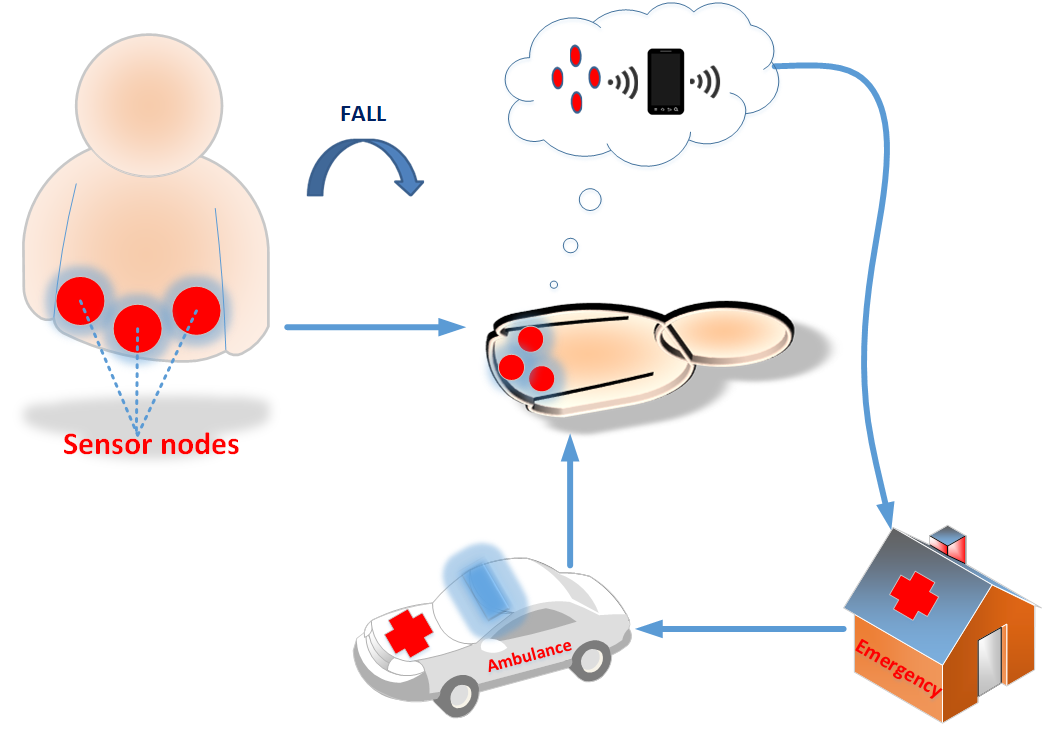
\includegraphics[scale=0.235]{Images/EscalationScheme.png}
	\caption[Escalation scheme]{Escalation scheme simulation~\cite{LaBlunda.2016,LaBlunda.2016b}}
	\label{fig:escalationscheme}
\end{figure}

A prototype in form of a belt has been developed which includes an electrocardiogram (ECG) harness and is based on a five sensor nodes Body Area Network (BAN). Each sensor node of the belt acquires continuously acceleration data including timestamp and the sensor node of the ECG harness provides the ECG signals including timestamp. In case of a fall the system should be capable to autonomously call the emergency services. Applying sensor fusion of physical and medical sensors we expect to improve the reliability of fall detection and possibly fall prevention. Another expectation is that the integration of medical sensors may facilitate the classification of different fall types. Detecting and classifying falls are critical in situations that may lead to loss of life if detected incorrectly. The BAN is generating a large amount of data in real time. Therefore data analysis technologies have to be used. Complex Event Processing (CEP) \cite{Esper:2016} is a data analysis technology which is used to manage and monitor in real time a huge volume of information that arrives in form of events with the lowest latency time. The CEP technology requires the usage of special software, the CEP engine. Each CEP technology provides a language called Event Process Languages (EPL). The EPL is used to detect relevant situations in real time by defining event patterns, in our case these relevant situations correspond to the detection of fall events. There are imperatives, rule-oriented and stream-oriented EPL types. For our research a stream-oriented EPL is used which will be introduced in Subsection \ref{subsec:CEP}.

Since testing the system plays an essential role in verifying the reliability of our fall detection prototype by simulating all possible fall events, the IoT-TEG tool \cite{Gutierrez2017,TesisGutierrez2017} is used. IoT-TEG \cite{Gutierrez2017,TesisGutierrez2017} is capable to automatically generate test events of any event type, so it can be adapted to different types of event falls.
With reference to the development of a reliable fall detection solution and the above mentioned expectations our ongoing research will be confronted with the following questions:
\begin{itemize}
	\item Will the integration of medical sensors improve the reliability of the fall detection system?
	\item Can the system achieve a high level of acceptance among people?	
\end{itemize}
% You must have at least 2 lines in the paragraph with the drop letter
% (should never be an issue)
The paper is structured as follows. Section \ref{sec:relatedwork} describes the related work regarding fall detection. In this section a short overview about existing solutions and different approaches for fall detection is given. Section \ref{sec:background} will describe the basic principles on which our ongoing fall detection research is based which contains the basic knowledge about falls, CEP \cite{Esper:2016} and IoT-TEG tool \cite{Gutierrez2017, TesisGutierrez2017}. In the successive section (Section \ref{sec:fall-detectionPrototype}) a detailed description of the fall detection prototype, including the generation of test events that includes the results of the fall analysis are introduced. Additionally, this section contains the usage of the ECG sensors and detected problems. Section \ref{sec:STAMP} will introduce the hazard analysis method STAMP \cite{leveson2011engineering} which is applied on the fall detection prototype. Section \ref{sec:FindingsResearchQuestions} discusses the findings of the research questions of our ongoing research. Finally, in Section \ref{sec:conclusion} a conclusion is given, including some indications for improvement which could be applied in the future work.

%\hfill mds
 
%\hfill August 26, 2015

\section{Related Work}
\label{sec:relatedwork}
In this section an overview about several fall detection approaches is given. There are several techniques which can be applied to detect fall events. Igual et al. \cite{Igual2013} illustrate the following different types of fall detection systems:
\begin{itemize}
	\item Context-aware systems
	\item Wearable systems
\end{itemize}
The functionality of context-aware systems depends on the environment, since the sensors and actuators must be installed in the living area (apartment, nursing home) in order to detect possible fall situations. The video-based context-aware solutions have the advantage to provide an accurate and reliable detection of falls with a fast assistance, but these systems have an issue regarding privacy. Patients using this solution are non-stop monitored limiting patient compliance. Additionally, the high purchase price is an obstacle for many patients and the dependency on the environment makes this approach useless in many application scenarios, because it would not detect fall events happening outside the networked area.

The other category of fall detection systems analyzed by Igual et al. \cite{Igual2013} contains wearable solutions worn on the body and are based on a BAN. This solution is capable to provide a fall detection which is independent from the environment in contrast to context-aware systems. The analysis of Igual et al. \cite{Igual2013} illustrates wearable fall detection systems using the sensor fusion with accelerometer and gyroscope data and built-in systems in form of smartphone sensors. For both categories of fall detection solutions (context-aware and wearable solution) several techniques were used. The following methods were applied for context-aware systems:
\begin{itemize}
	\item Image processing and threshold-based recognition
	\item Image processing and classification models
\end{itemize} 
The techniques used for the fall detection in wearable solutions are the following:
\begin{itemize}
	\item Threshold-based approach
	\item Fall detection based on machine learning based data analysis
\end{itemize}
Taking the fact into consideration that it is an essential advantage to focus on a wearable solution independent of external infrastructure, the work of Li et al.\cite{Li2009} serves as an example. Their solution includes two wearable sensor nodes which are based on a BAN. These sensor nodes consist of an accelerometer and gyroscope and they are placed on the chest (Node A) and on the thigh (Node B, see Figure \ref{fig:LietAl-Architecture}). 
\begin{figure}[!ht] 
	\centering
	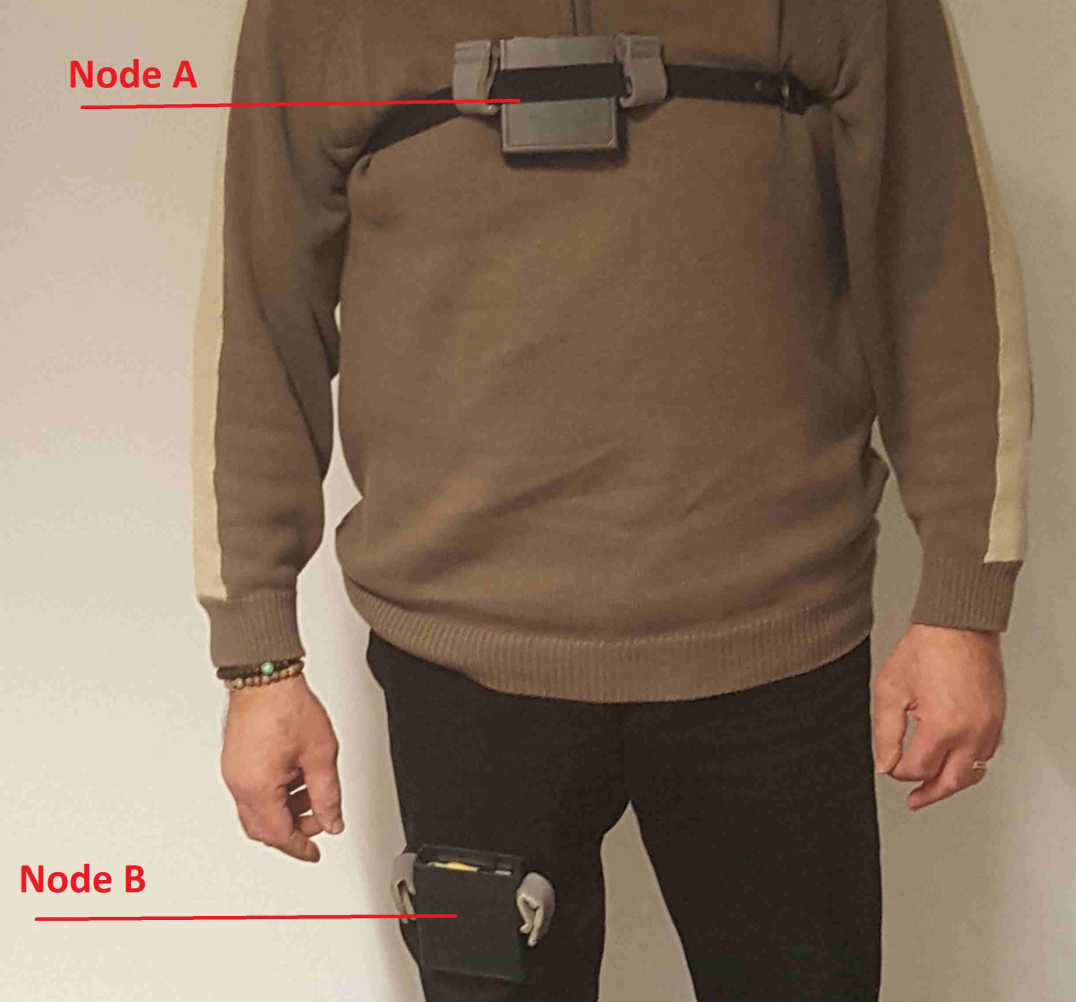
\includegraphics[scale=0.14]{Images/BasePrototype.png}
	\caption[System architecture according to Li et al.]{System architecture according to Li et al. \cite{Li2009}}
	\label{fig:LietAl-Architecture}
\end{figure}
The system distinguishes between two different motion sequences which are used for activity categorization: 
\begin{itemize}
	\item Static postures:
	\begin{itemize}
		\item Standing, sitting, lying
	\end{itemize}
	\item Dynamic postures:
	\begin{itemize}
		\item Activities of daily life (ADL) $\rightarrow$ walking, go up / down stairs, sit, jump, lay down, run
		\item Fall like motions $\rightarrow$ quick sit-down upright, quick sit-down reclined
		\item Flat surface falls $\rightarrow$ fall forward, fall backward, fall right, fall left
		\item Inclined falls $\rightarrow$ fall on stairs
	\end{itemize}
\end{itemize}
A 3-phase algorithm for fall detection is proposed by Li et al. \cite{Li2009}. The first phase of the fall detection algorithm examines if the person is in a static or dynamic position. If the analyzed position coincides with a static postures in the second phase it will be checked whether it corresponds to lying. If in lying position, it will be checked if the transition to this posture was intentional or unintentional (3\textsuperscript{rd} phase). To determine it, the previous 5 seconds of data is used. In the case it was unintentional the event will be classified as a fall. The proposed approach in \cite{Li2009} uses a threshold-based technique that is applied in the different phases of the algorithm. The weakness of this approach is to differentiate between activities of daily life and falling. Collado Villaverde et al. \cite{colladomachine} propose a wearable fall detection solution based on a smartwatch using acceleration data in combination with machine learning techniques.

A different approach to detect fall events is presented by Lüder et al. \cite{Luder2009} which apply an air pressure sensor in addition to the accelerometer. The hardware architecture proposed in \cite{Luder2009} depicts a wearable solution which is worn on the hip and provides wireless data transmission via Bluetooth. To take meteorological disturbances into account Lüder et al. \cite{Luder2009} incorporates an external barometric sensor as a reference. Another method for fall detection based on sensor fusion techniques is described by Gjoreski et al. \cite{Gjoreski2014}. Accelerometer and ECG data is used to detect fall events. The solution in \cite{Gjoreski2014} is capable of identifying person's movements and fall situations using wearable sensor nodes. These nodes are placed on the chest and thigh which is similar to Li et al's \cite{Li2009} approach. The advantage of the proposed solution by Gjoreski et al. \cite{Gjoreski2014} is the integration of medical sensors. The fusion of acceleration data and ECG signal facilitates the detection of anomalies in person's behavior and heart related problems that my lead to falls. According to their analysis differences in the ECG signal in different postures were detected. Lower beat rates in the static positions lying and sitting compared to walking were determined. Comparing the beat rates of both static postures (lying and sitting) differences were observed, where the beat rate of lying is lower than the one of sitting.

\section{Background}
\label{sec:background}

\subsection{Fall event analysis}
\label{subsec:fall-analysis}
The fall detection prototype is based on the approach proposed in \cite{Gjoreski2014, Kozina}. To detect a fall event a typical physical behavior is used which comprises the following phases:
\begin{itemize}
	\item Prefall phase 
	\item Falling phase
	\item Impact phase
	\item Postfall phase
\end{itemize}
The Figure \ref{fig:fallKozina} shows the mentioned phases. The prefall phase illustrates a stationary position of the person where the measured acceleration is around 1g (9.81$m/s^{2}$). During the free falling phase the  acceleration decreases close to 0g (0$m/s^{2}$). Upon the impact, the acceleration reaches his maximum value for a short period of time. Subsequently, the acceleration is decreasing to around 1g (9.81$m/s^{2}$) which represents the postfall lying phase. To apply this fall detection pattern the accelerometer data is used. For the impact detection the acceleration magnitude is used which is calculated with eq. \ref{eq:acel} and to determine the body's orientation the single axis values of the accelerometer ($\alpha_x$, $\alpha_y$, $\alpha_z$) are analyzed:

\begin{equation}\label{eq:acel}
\alpha = \sqrt{\alpha_{x}^{2} + \alpha_{y}^{2} + \alpha_{z}^{2}}
\end{equation}

\begin{figure}[!ht]
	\centering
	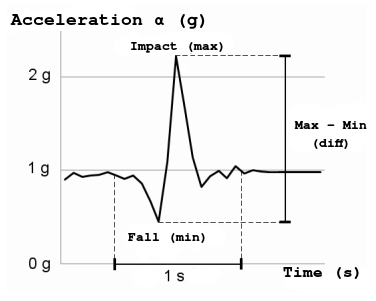
\includegraphics[scale=0.5]{Images/FallGraph}
	\caption[Acceleration during impact]{Acceleration during impact according to Kozina et al.~\cite{Kozina}}
	\label{fig:fallKozina}
\end{figure}
 Assuming that the person is in a standing position (static posture), the x-acceleration ($\alpha_x$) corresponds to 1g (9.81$m/s^{2}$) and the other two axis ($\alpha_y$, $\alpha_z$) would be close to 0g (0$m/s^{2}$). As soon as the person changes his posture, the gravitational force will act on one of the other two axis ($\alpha_y$, $\alpha_z$) and the x-acceleration will be 0g (0$m/s^{2}$). Combining this information with the acceleration magnitude (see Formula \ref{eq:acel}) the system is able to detect the fall and additionally determine the type of fall. For applying this knowledge the EPL of EsperTech (Esper EPL from now on) \cite{Esper:2016} was used.

To ensure reliable fall detection, the system must be able to detect various types of falls. For this reason, the development of the fall detection prototype is also based on the creation of a test protocol covering different types of falls. Li et al. \cite{Li2009} and Pannurat et al. \cite{Pannurat2014} are our references, as they not only represent possible solutions for fall detection, but also offer a versatile overview of possible fall scenarios.

\subsection{Fall patterns based on Esper EPL}
\label{subsec:CEP}
The EPL used is the Esper EPL \cite{Esper:2016}, which is a streaming-oriented language and uses the CEP engine to execute the queries. The main reasons for its usage are the following:
\begin{itemize}
	\item The syntax is based on SQL $\rightarrow$ complex events can be easily formulated.
	\item It can be embedded in Java applications.
	\item It is open-source.
	\item CEP engine of EsperTech processes around 500.000 events per second on a workstation and between 70.000 and 200.000 events per second on a notebook (according to its developer) $\rightarrow$ This is an essential feature to simulate time-critical applications. 
\end{itemize}
In comparison to SQL, which is based on tables, EPL works on the continuously incoming data stream. Therefore, a row from a SQL table corresponds to an event in the event stream. 

To define rules in CEP the incoming event should be characterized in detail to specify incoming data for the CEP-engine. After the event creation, rules, as well called event patterns, should be determined to categorize the incoming input in fall events or daily activities.
\renewcommand{\lstlistingname}{Example}
\begin{lstlisting}[basicstyle=\ttfamily\footnotesize,language=SQL,caption=Fall pattern based on Kozina et al. \cite{Kozina},label=CEPPattern, breaklines=true]
//1. Definition of the event - incoming data for CEP
*---------------------------------------------*
create schema BodyEvent(PersonID integer,accelS1 double,accelS2 double,timestamp string)

//2. Definition of Event pattern
*---------------------------------------------*
select a1.accelS1, a2.accelS1, a1.accelS2, a2.accelS2 from pattern [every(a1=BodyEvent(a1.accelS1 <= 9.81) -> a2=BodyEvent(a2.accelS1-a1.accelS1 >= 9.81 and a1.PersonID = a2.PersonID) where timer:within(1sec)) or every (a1=BodyEvent(a1.accelS2 <= 9.81)-> a2=BodyEvent(a2.accelS2-a1.accelS2 >= 9.81 and a1.PersonID = a2.PersonID) where timer:within(1sec))];
\end{lstlisting}

The illustrated EPL query (see Example \ref{CEPPattern}) is based on the physical principle shown in Figure \ref{fig:fallKozina} (see Subsection \ref{subsec:fall-analysis}). It should be highlighted, that two nodes were used for this EPL query (one frontal node and one lateral node) to apply the fall detection, but in future this query will be extended for all the sensor nodes of our prototype BAN. The four nodes BAN architecture is currently only used for redundancy purposes. In the Example \ref{CEPPattern} the following event properties are used for the definition of the event pattern:
\begin{itemize}
	\item a1.accelS1 $\rightarrow$ initial acceleration value of sensor node 1.
	\item a2.accelS1 $\rightarrow$ successive acceleration value of sensor node 1.
	\item a1.accelS2 $\rightarrow$ initial acceleration value of sensor node 2.
	\item a2.accelS2 $\rightarrow$ successive acceleration value of sensor node 2.
\end{itemize}
Referring to the selected properties this example checks, if the initial acceleration of node 1 (a1.accelS1) is $<= 9.81$ m/$s^2$ which indicate that the person is in a stationary position. Subsequently, it will be checked if the difference of the successive acceleration (a2.accelS1) and the first acceleration (a1.accelS1) within 1 second is $>= 9.81$ m/$s^2$. If this condition is fulfilled, it is an indication that the person has suffered an impact. Adding the OR disjunction the second sensor node can be integrated and the statement is able to detect a fall in case one of the node's data matches the Esper EPL query and the values of the acceleration correspond to the same person.

\subsection{IoT test event generator}
\label{iotteg}

IoT-TEG~\cite{Gutierrez2017,TesisGutierrez2017} is a Java-based tool which takes an event 
type definition file and a desired output format JSON, CSV and XML, the most common across IoT platforms. IoT-TEG is made up of a \emph{validator} and an \emph{event generator} 
(Figure~\ref{fig:IoT-EGArquitecture}). The validator ensures the definition follows the rules set 
by IoT-TEG. The generator takes the definition and generates the indicated number of events according to it.

\begin{figure}[!ht]
	\centering
	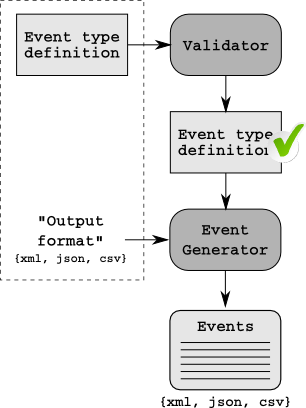
\includegraphics[scale=0.445]{Images/IoT-EGArquitecture}
	\caption[IoT-TEG Architecture]{IoT-TEG Architecture~\cite{TesisGutierrez2017,Gutierrez2017}.}
	\label{fig:IoT-EGArquitecture}
\end{figure}
Previous studies suggested there were no differences in testing effectiveness between using events
generated by IoT-TEG, or events recorded from various case studies~\cite{Gutierrez2017,TesisGutierrez2017}.
Moreover, thanks to its implementation, IoT-TEG can be used to do different type of test: functional,
negative, integration, stress, etc; indeed an example of its usability can be found 
in~\cite{TesisGutierrez2017,gutierrez2018}, where IoT-TEG has been used to apply mutation 
testing~\cite{jia2011}. These results confirm IoT-TEG can 
simulate many types of events occurring in any type of applications, it can do different type of tests
and it can solve the main challenges developers face when they test event-processing programs: lack of data for testing, needing specific values for the events, and needing the source to generate the events.
For the sake of clarity, Example~\ref{eventTypeDef} shows an event type
definition.
\begin{lstlisting}[basicstyle=\ttfamily\footnotesize,language=XML,caption=Event type definition example,label=eventTypeDef, breaklines=true]
<?xml version="1.0" encoding="UTF-8"?>
<event_type name="TemperatureEvent">
<block name="feeds" repeat="150">
<field name="created_at" quotes="true" type="ComplexType">
 <attribute type="Date" format="MM-dd"></attribute>
 <attribute type="String" format="T"></attribute>
 <attribute type="Time" format="hh:mm"></attribute>
</field>
<field name="entry_id" quotes="false" type="Integer" min="0" max="10000"></field>
<field name="temp" quotes="false" type="Float" min="0" max="500" precision="1"></field>
</block>
</event_type>
\end{lstlisting}

The defined event type contains three properties: \texttt{created\_at},
\texttt{entry\_id} and \texttt{temp}. These properties are defined as
fields in the event type definition. The \texttt{created\_at} field is complex
type and \texttt{entry\_id} and \texttt{temp} are simple types. 

Apart from the mentioned challenges that IoT-TEG solves in order to test 
event-processing programs, it incorporates a specific functionality
for testing programs that use the Esper EPL \cite{Esper:2016}. 
This functionality helps to 
automatically generate events with specific values in accordance with the 
program which will process them. IoT-TEG analyses the Esper EPL queries and 
generates events depending on the logical and relational operations. 

% needed in second column of first page if using \IEEEpubid
%\IEEEpubidadjcol

\section{Fall detection system prototype}
\label{sec:fall-detectionPrototype}	

\subsection{Architecture}
\label{subsec:Architecture}	
 A first prototype was described in \cite{LaBlunda.2016, LaBlunda.2016b}. This paper presents an improved version of the prototype in \cite{LaBlunda.2016, LaBlunda.2016b}, which includes essential developments that contribute to reliable operation of the system. Additionally, the improved hardware design meets the requirement for patient compliance. A more user friendly design facilitates the freedom of movement for the user. As a safety critical system for medical purposes, a redundant hardware design protects the system against a total system failure which would have severe consequences in case of fall events. Referring to J{\"a}ms{\"a} et al. \cite{jamsa2014fall} the best approach is to position the accelerometer near to the waist. Taking into consideration these aspects a wearable belt solution was developed which is based on a four sensor nodes BAN (see Figure \ref{fig:BanBelt}). The four sensor nodes (S1 - S4) positioned on the belt are acting as peripherals and are continuously acquiring acceleration data which is sent via Bluetooth Low Energy (BLE) to the smartphone (central device). 
\begin{figure}[!ht]
	\centering
	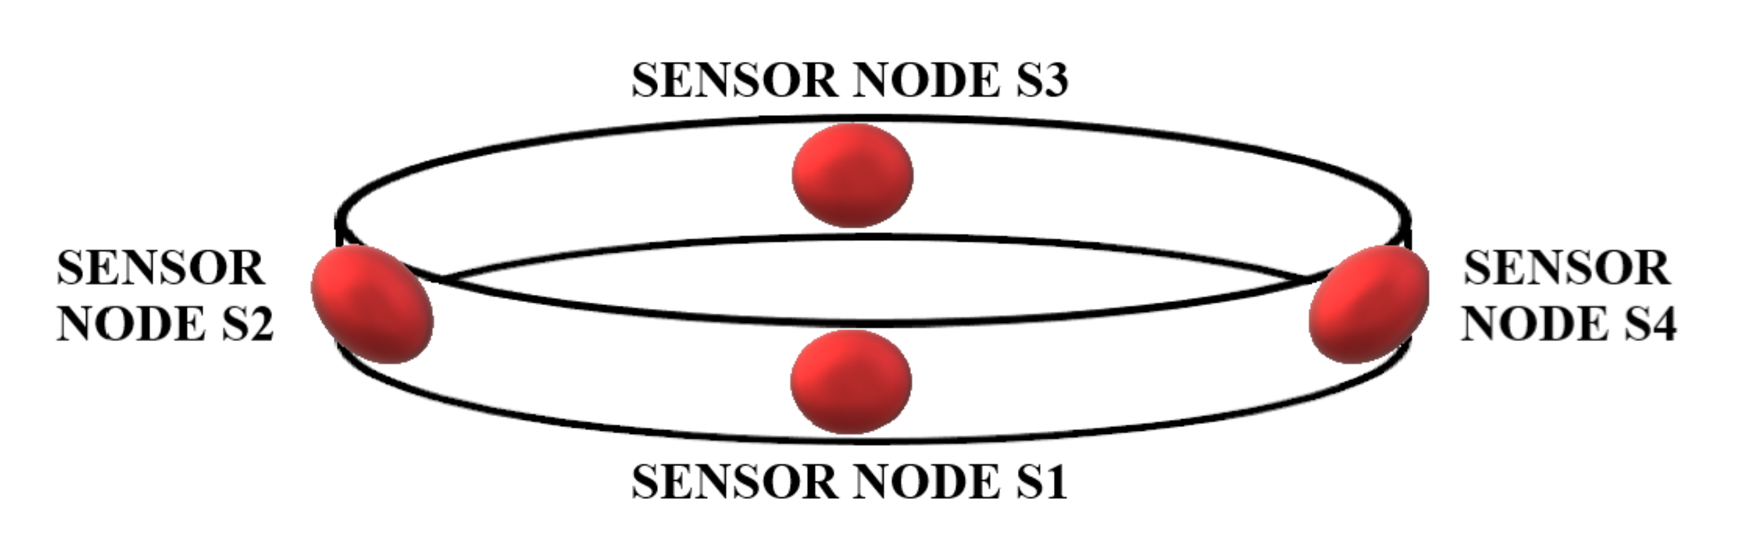
\includegraphics[scale=0.27]{Images/belt.eps}
	\caption[Four sensor nodes BAN - Belt]{Four sensor nodes BAN - Belt \cite{LaBlunda.2016, LaBlunda.2016b}}
	\label{fig:BanBelt}
\end{figure}

The dataset consists of the following information: 
\begin{center}
	SensorID, $\alpha_{x}$, $\alpha_{y}$, $\alpha_{z}$ measured in m/$s^2$
\end{center}
\begin{itemize}
	\item \textbf{SensorID} $\rightarrow$ sensor node identification.
	\item \boldmath{$\alpha_{x}$} $\rightarrow$ acceleration value in X-direction.
	\item \boldmath{$\alpha_{y}$} $\rightarrow$ acceleration value in Y-direction.
	\item \boldmath{$\alpha_{z}$} $\rightarrow$ acceleration value in Z-direction.
\end{itemize} 
The central device receives the incoming sensor data which will be stored in separate data files to evaluate the event. 
The belt solution reflects the above criteria of a safety critical systems. The proposed architecture (see Figure \ref{fig:BanBelt}) is based on a mirroring principle of the opposite sensor nodes which provide identical acceleration values, only with different signs. If a sensor node fails during operation, the opposite node can be used as a reference to ensure accurate evaluation of the event.  Considering the following scheme (see Figure \ref{fig:ReferenceScheme}) this fall detection belt solution facilitates the recognition of different fall event types. The positioning of the nodes around the hip allows a precise fall characterization.
\begin{figure}[!ht]
	\centering
	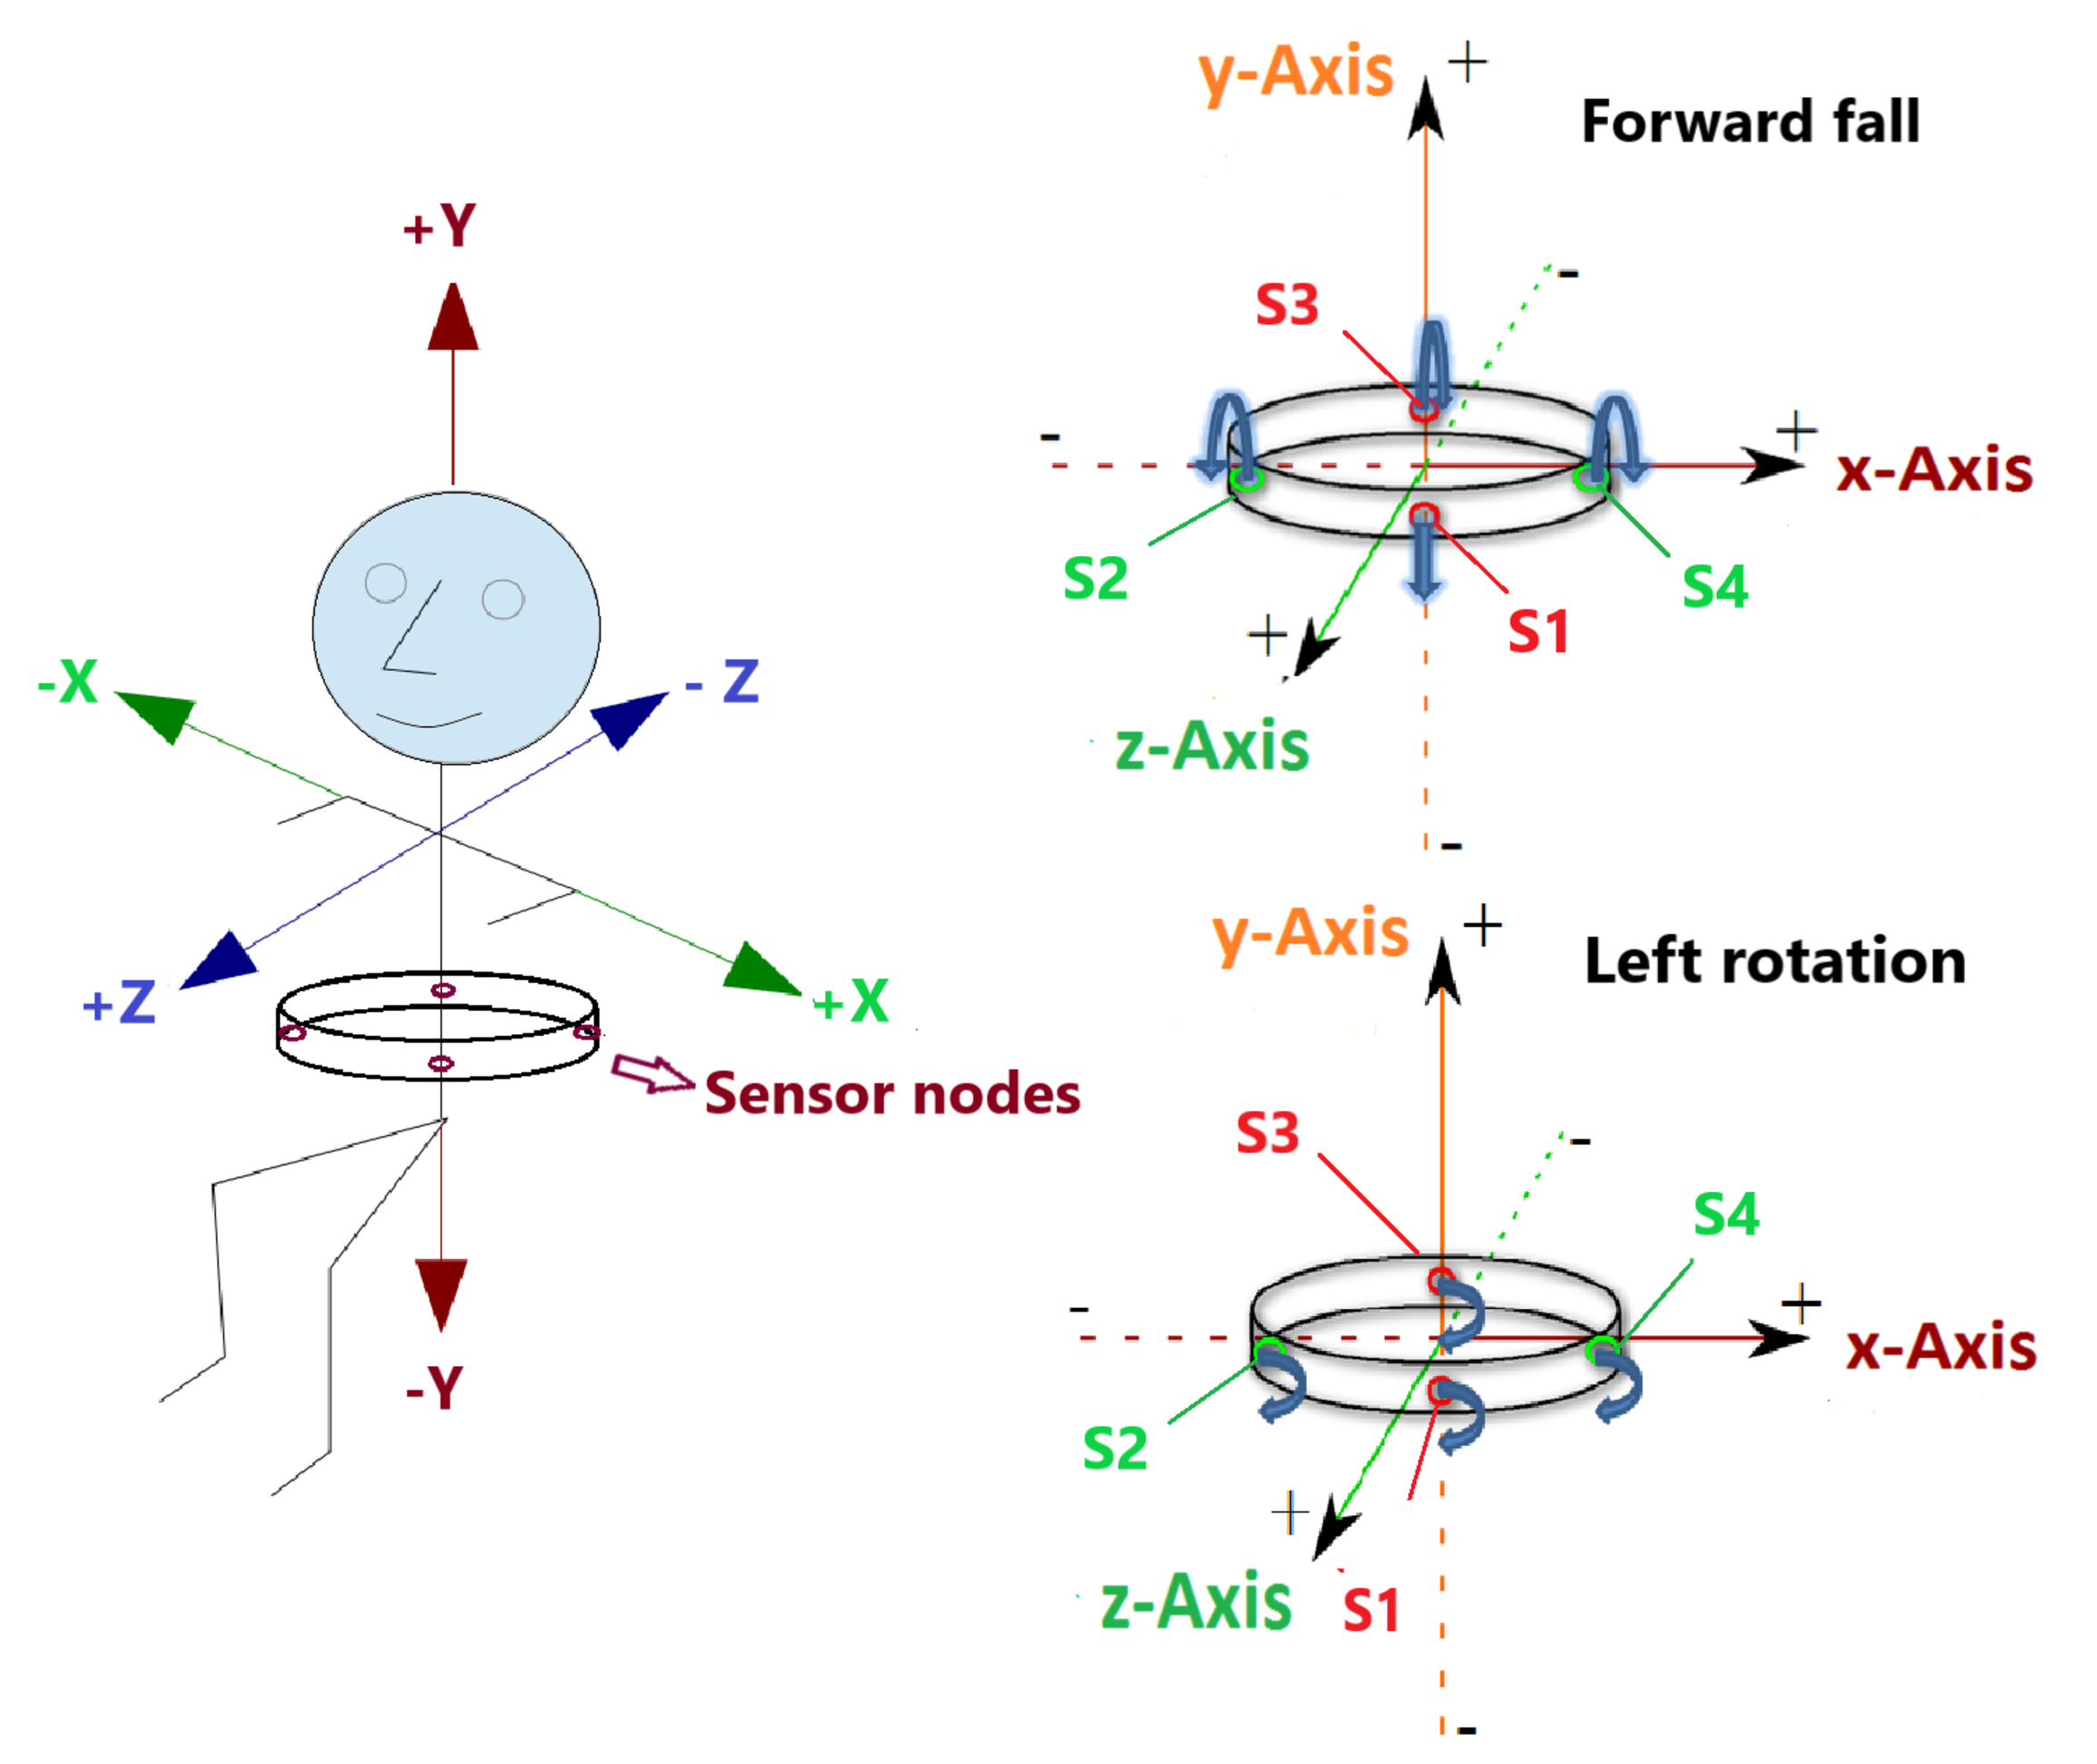
\includegraphics[scale=0.19]{Images/axis.eps}
	\caption[Three axis reference scheme]{Three axis reference scheme \cite{LaBlunda.2016,LuigiMasterThesis}}
	\label{fig:ReferenceScheme}
\end{figure}

Fall type example: a person suffering a multi phase frontal fall because of a fainting. Analyzing the fall event, it can be determined that the fall caused originally by fainting leads firstly to a left rotation of the person's body (prefall phase). In  the next phase the forward fall results in the person’s impact
to the ground. Projecting this fall event on the reference scheme (see Figure \ref{fig:ReferenceScheme}), the body's orientation (e.g. left rotation) can be determined on the basis of the individual acceleration values ($\alpha_x$,  $\alpha_y$,  $\alpha_z$). Additionally, the acceleration magnitude (see Formula \ref{eq:acel}) can be used for the detection of the impact which is categorized by a temporary increase in the acceleration, as described in the previous Section \ref{sec:background}. Using the Esper EPL query (Example \ref{CEPPattern}) stated in the Subsection \ref{subsec:CEP} the system is capable to detect a general fall event based on the physical principle proposed by \cite{Kozina}.
Taking into consideration the test protocol stated in Section \ref{sec:background} typical fall events (e.g. rolling out of the bed) in nursing homes and hospitals can be detected by this solution. In the subsequent subsection, the behavioral analysis of the acceleration values during one of the mentioned typical fall events is presented, the \textit{fall against wall} (FAW). Additionally, test events are generated to simulate the FAW fall type.

\subsection{Fall simulation test events}

The fall to generate the test events consists on the impact of the person with 
a wall and falling on the knees and then on the chest: FAW. 
In this study we have used two healthy subjects, and we have recorded falls with all 
possible realism while also trying to avoid risks. They have been doing FAW fall test for a period 
of 2 minutes. The analyzed data and videos can be found in~\cite{FallRepo}.
In this analysis the following steps have been done:

\subsubsection{Study of the values} Given that the sensor (S1) is the one that suffers the 
impact, its acceleration values are the first to be analyzed. The goal is to study 
the acceleration behavior during a fall in order to generate test events, so the acceleration 
values are normalized ($N(m/s^2)$). After the normalization the impact, peaks, 
have to be detected; we have considered a peak when the normalized acceleration is 
greater than 0,7 ($N(m/s^2) > 0,7$). 

While performing the data analysis, it has to be taken into account that the values suffer 
alterations because several factors: the person movement, the person bounces against something 
(floor, wall, etc), the collocation of the sensors to the original position after a fall, 
sensor pressure because an impact or the person is laying over it, etc.

After applying the previous rule in all the fall data and taking into account the alterations 
because the mentioned factors, the impacts are detected.

\subsubsection{Fall identification and analysis} Once the peaks are detected, a range of values, 
including the peaks, are selected in order to analyse data properly and to study the acceleration 
behavior during FAW fall. The range of extracted values is a set of data that happens in less 
than a time window of 1 second, to meet the fall rule of~\cite{Luder2009} described in eq. \ref{eq:acel}, see Section~\ref{sec:background}. 
%The Table~\ref{tabla:FAW} shows the acceleration value during one FAW fall of person 1 and person 2. 

%\begin{table}[!ht]
%	\centering
%	\caption{FAW fall acceleration, person 1 and 2}%
%	\label{tabla:FAW}
%	\begin{tabular}{*{5}{r}}
%		\centering
\begin{tabularx}{9.5cm}{@{}ccc|ccc@{}}
  \toprule
  \multicolumn{1}{p{0.65cm}}{\centering \textsc{Time} \\ ($s.ms$)} & \multicolumn{1}{p{0.65cm}}{\centering \textsc{Accel.} \\ ($m/s^2$)} & \multicolumn{1}{p{2cm}}{\centering \textsc{N. Accel.} \\ ($N(m/s^2)$)} & \multicolumn{1}{p{0.65cm}}{\centering \textsc{Time} \\ ($s.ms$)} & \multicolumn{1}{p{0.65cm}}{\centering \textsc{Accel.} \\ ($m/s^2$)}& \multicolumn{1}{p{2cm}}{\centering \textsc{N. Accel.} \\ ($N(m/s^2)$)} \\
  \midrule
57.311 & 3,63 & 0,01 & 25.254 & 8,53 & 0,09 \\
57.359 & 3,43 & 0,00 & 25.303 & 10,79 & 0,19 \\
57.408 & 7,85 & 0,17 & 25.352 & 11,28 & 0,22 \\
57.506 & 10,99 & 0,30 & 25.401 & 13,83 & 0,34 \\
57.506 & 6,47 & 0,12 & 25.449 & 9,42 & 0,13 \\
57.554 & 4,61 & 0,05 & 25.503 & 8,63 & 0,09 \\
57.603 & 4,22 & 0,03 & 25.546 & 0,89 & 0,10 \\
57.651 & 22,86 & {\setlength{\fboxsep}{0pt}\colorbox{bananayellow}{0,77}} & 25.596 & 8,04 & 0,07 \\
57.700 & 28,84 & {\setlength{\fboxsep}{0pt}\colorbox{bananayellow}{1,00}} & 25.645 & 13,93 & 0,35 \\
57.749 & 21,78 & {\setlength{\fboxsep}{0pt}\colorbox{bananayellow}{0,72}} & 25.693 & 22,7 & {\setlength{\fboxsep}{0pt}\colorbox{bananayellow}{0,76}} \\
57.800 & 9,03 & 0,22 & 25.742 & 10,59 & 0,19 \\
57.846 & 10,79 & 0,29 & 25.791 & 8,63 & 0,09 \\
57.900 & 10,79 & 0,29 & 25.841 & 8,34 & 0,08 \\
57.944 & 9,32 & 0,23 & 25.888 & 6,67 & 0,00 \\
57.996 & 13,15 & 0,38 & 25.937 & 17,46 & 0,51 \\
58.042 & 20,99 & 0,69 & 25.986 & 27,76 & {\setlength{\fboxsep}{0pt}\colorbox{bananayellow}{1,00}} \\
58.186 & 28,25 & {\setlength{\fboxsep}{0pt}\colorbox{bananayellow}{0,98}} & 26.082 & 11,58 & 0,23 \\
58.188 & 27,47 & {\setlength{\fboxsep}{0pt}\colorbox{bananayellow}{0,95}} & 26.084 & 11,38 & 0,22 \\
58.240 & 10 & 0,26 & 26.134 & 10,5 & 0,18 \\
58.286 & 10,99 & 0,30 & 26.181 & 8,83 & 0,10 \\
58.334 & 11,67 & 0,33 & 26.230 & 12,75 & 0,29 \\
  \bottomrule
\end{tabularx}


%	\end{tabular}
%\end{table}

%The first and fourth columns of the Table~\ref{tabla:FAW} represent the seconds and milliseconds ($s.ms$) when the acceleration was measured. The second and fifth columns show the acceleration values ($m/s^2$) and in the third and sixth columns are deployed the normalized acceleration values 
%($N(m/s^2)$) according to the fall maximum value. 
Figure~\ref{fig:FAWcomparison} confronts the normalized acceleration behavior during the previous FAW falls of person 1 and person 2. These comparisons show a similar behavior of the acceleration during the FAW fall.
\begin{figure}[!ht]
	\centering
	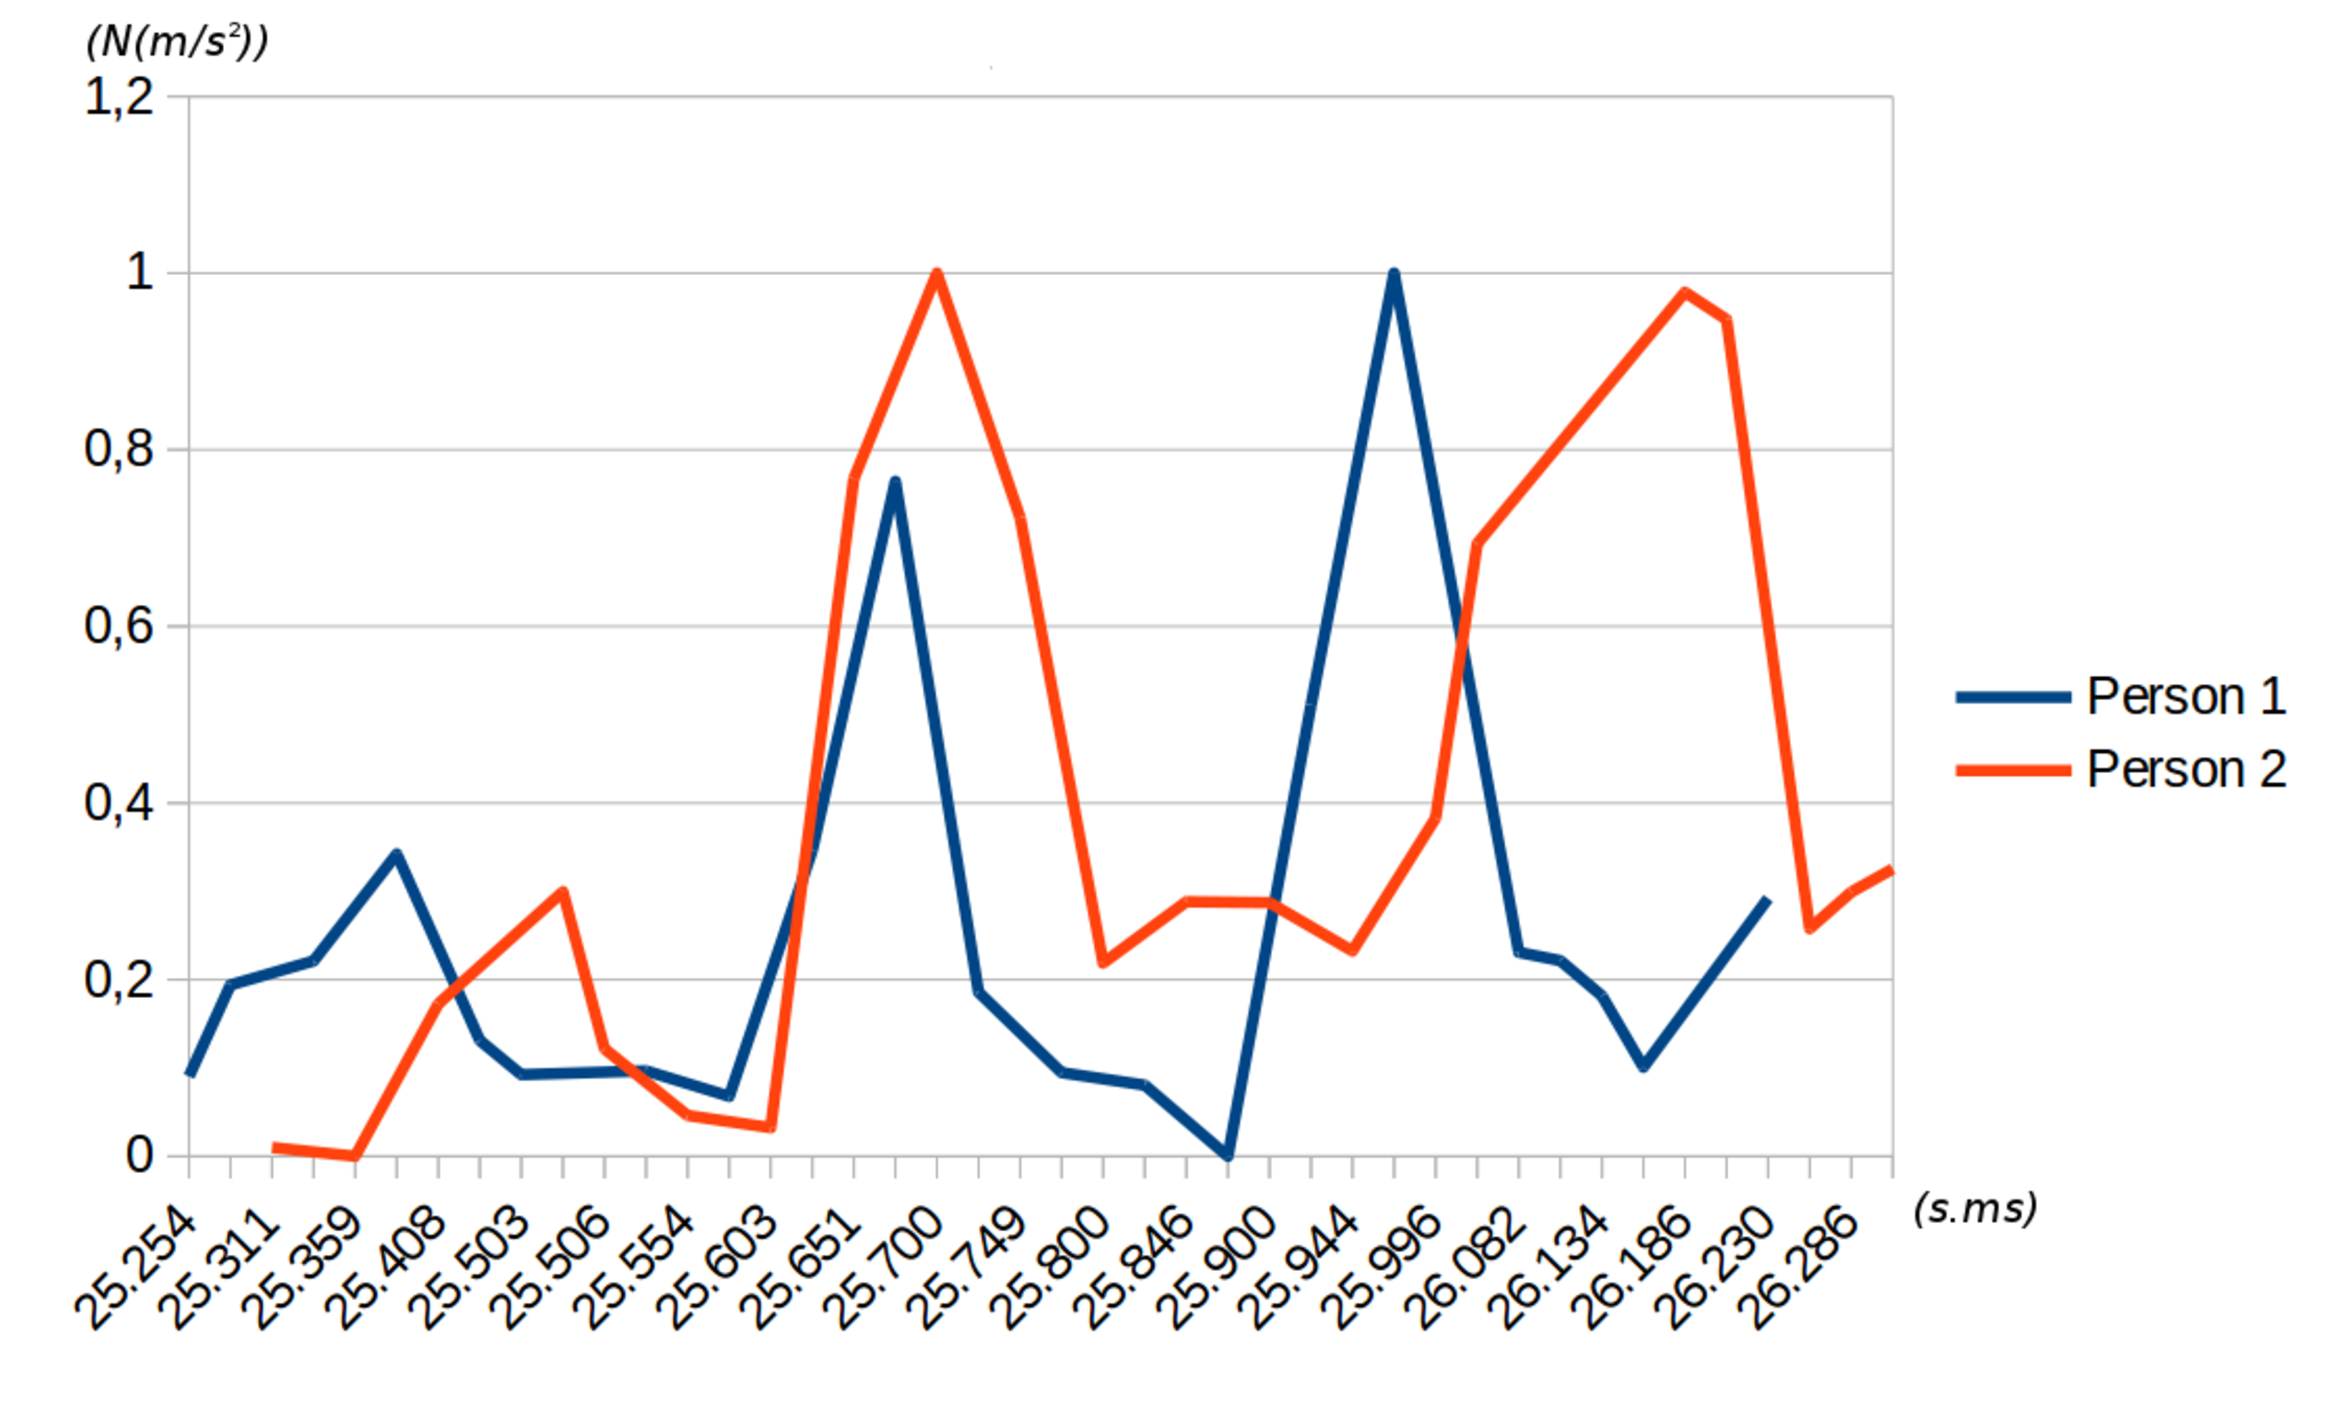
\includegraphics[scale=0.21]{Images/TwoFallsComparative.eps}
	\caption[Acceleration during FAW fall]{Acceleration comparison during FAW fall.}
	\label{fig:FAWcomparison}
\end{figure}

We have decided to define the acceleration behavior with normalized values; so the normalized acceleration behavior during the FAW consists on:
\begin{enumerate}
	\item The variation of its values while the person is walking. We have divided this rule in two rules:
	\begin{enumerate}
		\item The normalized acceleration values go increasing in a range [0, 0.35].
		\item The normalized acceleration values go decreasing in a range [0, 0.35].
	\end{enumerate}
	\item As a consequence of the impact of the person against a wall, the acceleration normalized value has to be greater than 0.7.
	\item The normalized acceleration values decrease to a range [0, 0.35]. The values of the acceleration are in the mentioned range depending on the size of the person; the larger person results in a longer range and if the person retains a position prior to a fall thanks to the wall. Moreover, a subtle peak could appear as a consequence of a rebound.
	\item A second impact happens when the person hit the ground, the acceleration normalized values have to be greater than 0.7.
	\item Finally, the person is laying on the ground and the normalized acceleration value decreases. The values of the acceleration are between [0.10, 0.35] and no subtle peaks appear. 
\end{enumerate}
The same analysis process has been done to the rest of sensors, and the acceleration follows the same pattern.

\subsubsection{To define the fall event} Once the fall acceleration behavior has been observed, the next step is to define the 
fall event in order to generate test events with IoT-TEG~\cite{TesisGutierrez2017,Gutierrez2017}. As it was explained in 
Subsection~\ref{iotteg}, the event type attributes have
to be defined using the \texttt{<field>} element. The fall event contains one attribute, the acceleration, which is float, 
\texttt{type=``Float''}, and its values are not quoted, \texttt{quotes=``false''}. A new parameter in IoT-TEG has been defined as a 
consequence of the previous fall study. Given that the acceleration values follow a specific behavior, it is necessary to include 
the \texttt{custom\_behavior} property in the \texttt{<field>} element to define the behavior of any event attribute; 
in this study, the acceleration. In the \texttt{custom\_behavior} property the path to the file that includes the behavior of the 
event attribute has to be written. The Example~\ref{FallEvent} shows the complete fall event definition (FallEventType).

\begin{lstlisting}[basicstyle=\ttfamily\footnotesize,language=XML,caption={Fall event type definition},label=FallEvent, breaklines=true]
<?xml version="1.0" encoding="UTF-8"?>
<event name="FallEventType">
<block name="feeds" repeat="100">
<field name="acceleration" quotes="false" type="Float" custom_behavior="/Path/To/Rule/File">
</field>
</block>
</event>
\end{lstlisting}

IoT-TEG includes a new functionality, which has been implemented to simulate the desired behavior of an event attribute with a \texttt{custom\_behavior} property in its event type definition. This functionality allows to generate values of the event attribute following a behavior that the user has described in a file.
In order to explain how the user has to define the desired behavior of an event attribute, we are going to use the FAW fall behavior rules (see Example~\ref{FAWFallRules}). In a XML file the number of simulations has to be
indicated, the events involved in a simulation will be calculated according to the total number of events to generate and the desired simulations. For example, if the number of test events to generate is 100, number indicated in the event type definition file, \texttt{repeat="100"}, and the number of desired 
simulations is 5, \texttt{simulations="5"}, number indicated in the behavior rules definition file, the number of events to simulate the behavior is 20. In Example~\ref{FAWFallRules}, the user ask to generate 100 test events and 5 falls (simulations), so 20 events will be used to define a FAW fall.

Variables can be defined if they are needed in the behavior rules. They can be defined in the file where the behavior rules are included using the \texttt{<variables>} tags. To define them a name and a value 
have to be given to the variables. The value can be defined as a fixed value with the \texttt{value} property, or using a range with the \texttt{min} and \texttt{max} properties. Moreover, in some variables
are involved in the value of another variables; this is indicated using the variable with an specific format \texttt{\$(variable)}, see Example~\ref{FAWFallRules}. In addition, arithmetic operations can be done in the definition of the variable values. Let us see how using them in the FAW fall example. To define the acceleration behavior during a FAW fall three variables are defined: \texttt{Base}, 
\texttt{ImpactWall} and \texttt{Impact}. Given that the acceleration behavior during a FAW fall has being done according to the normalized values, the variables and rules have been defined according to that analysis. The acceleration value in a stationary position is variable depending on the person, so we have considered the established value, $1g\approx9.81m/s^{2}$. That is the fixed value of the \texttt{Base} variable. To determine the values of the impacts, we have taken into account that the 
normalized value have to be $> 0,7$. So, to ensure that the impacts, \texttt{ImpactWall} and \texttt{Impact}, have a value meeting the mentioned condition the minimum value of the impact is the sum of the \texttt{Base} and \texttt{Base} multiply by \texttt{Base}$*0,7$; and the maximum value of the impacts is $3g\approx9,81*3=$\texttt{Base}$*3$.

Once the variables are defined, the rules have to be determined. The first step is to indicate the \texttt{weight} for each rule in order to calculate the number of events to generate for each rule for each simulation. Following the simulation values the number of events to generate for each rule, according to the assigned weights, is: $20 * 0,25 = 5$ events will be generated for the first rule, another 5 events 
for the second rule, 1 event for the third rule, 5 events for the fourth rule, 1 event for the fifth rule and the remaining events, three events, for the sixth rule. We have to assign zero to the weight \texttt{weight="0"} to indicate how the remaining events have to be generated.

To define the rules, \texttt{min}, \texttt{max} and \texttt{value} properties can be used as well as the arithmetic operations and the references to another variables. Moreover, the \texttt{sequence} property can be used to obtain values lower or higher than the one generated previously: \texttt{inc}, to increase the value, or \texttt{dec}, to decrease the value. 

\begin{lstlisting}[basicstyle=\ttfamily\footnotesize,language=XML,caption={Rules to define a FAW fall},label=FAWFallRules, breaklines=true]
<?xml version="1.0" encoding="UTF-8"?>
<custom_conditions simulations="5">
<variables>
<variable name="Base" value="9.81"/>
<variable name="ImpactWall" min="$(Base)+$(Base)*0.7" max="$(Base)*3"/>
<variable name="Impact" min="$(Base)+$(Base)*0.7" max="$(Base)*3"/>
</variables>
<rules>
<rule weight="0.25" min="0" max="$(ImpactWall)*0.35" sequence="inc"/>
<rule weight="0.25" min="0" max="$(ImpactWall)*0.35" sequence="dec"/>
<rule weight="1" value="$(ImpactWall)"/>
<rule weight="0.25" min="0" max="$(Impact)*0.35"/>
<rule weight="1" value="$(Impact)"/>
<rule weight="0" min="$(Base)+$(Base)*0.10"
max="$(Impact)*0.35"/>
</rules>
</custom_conditions>
\end{lstlisting}

Thanks to the included properties and parameters in the IoT-TEG new functionality, the desired behavior rules that
follow the normalized acceleration values can be defined. Given that we have considered to define the FAW fall behavior
rules according to the normalized values, the values to generate depend on the maximum value. Due to there are two 
values that can be the highest one, \texttt{ImpactWall} or \texttt{Impact}, the rules that depend on the maximum 
value contains the reference to the value, \texttt{ImpactWall} or \texttt{Impact}, according to the proximity
of the rule. For instance, the first and second FAW fall rules contain a reference to \texttt{ImpactWall}, the impact 
in the wall (third rule), which happens after the person is walking, something described in the first and the second rules.
The fourth and sixth rules contain a reference to \texttt{Impact}, the impact on the ground (fifth rule), which happen
after the person is falling and the person is laying on the floor, fourth and sixth rules.

It is needed to highlight that to obtain these rules to define the behavior of the normalized acceleration several test have been done. Once we obtained the desired results, test events were generated as they were necessary. The Figure~\ref{fig:IoTTEGFAWGeneratedEvents} shows the acceleration values of some of the generated FAW falls using IoT-TEG and the new functionality.

\begin{figure}[!ht]
	\centering
	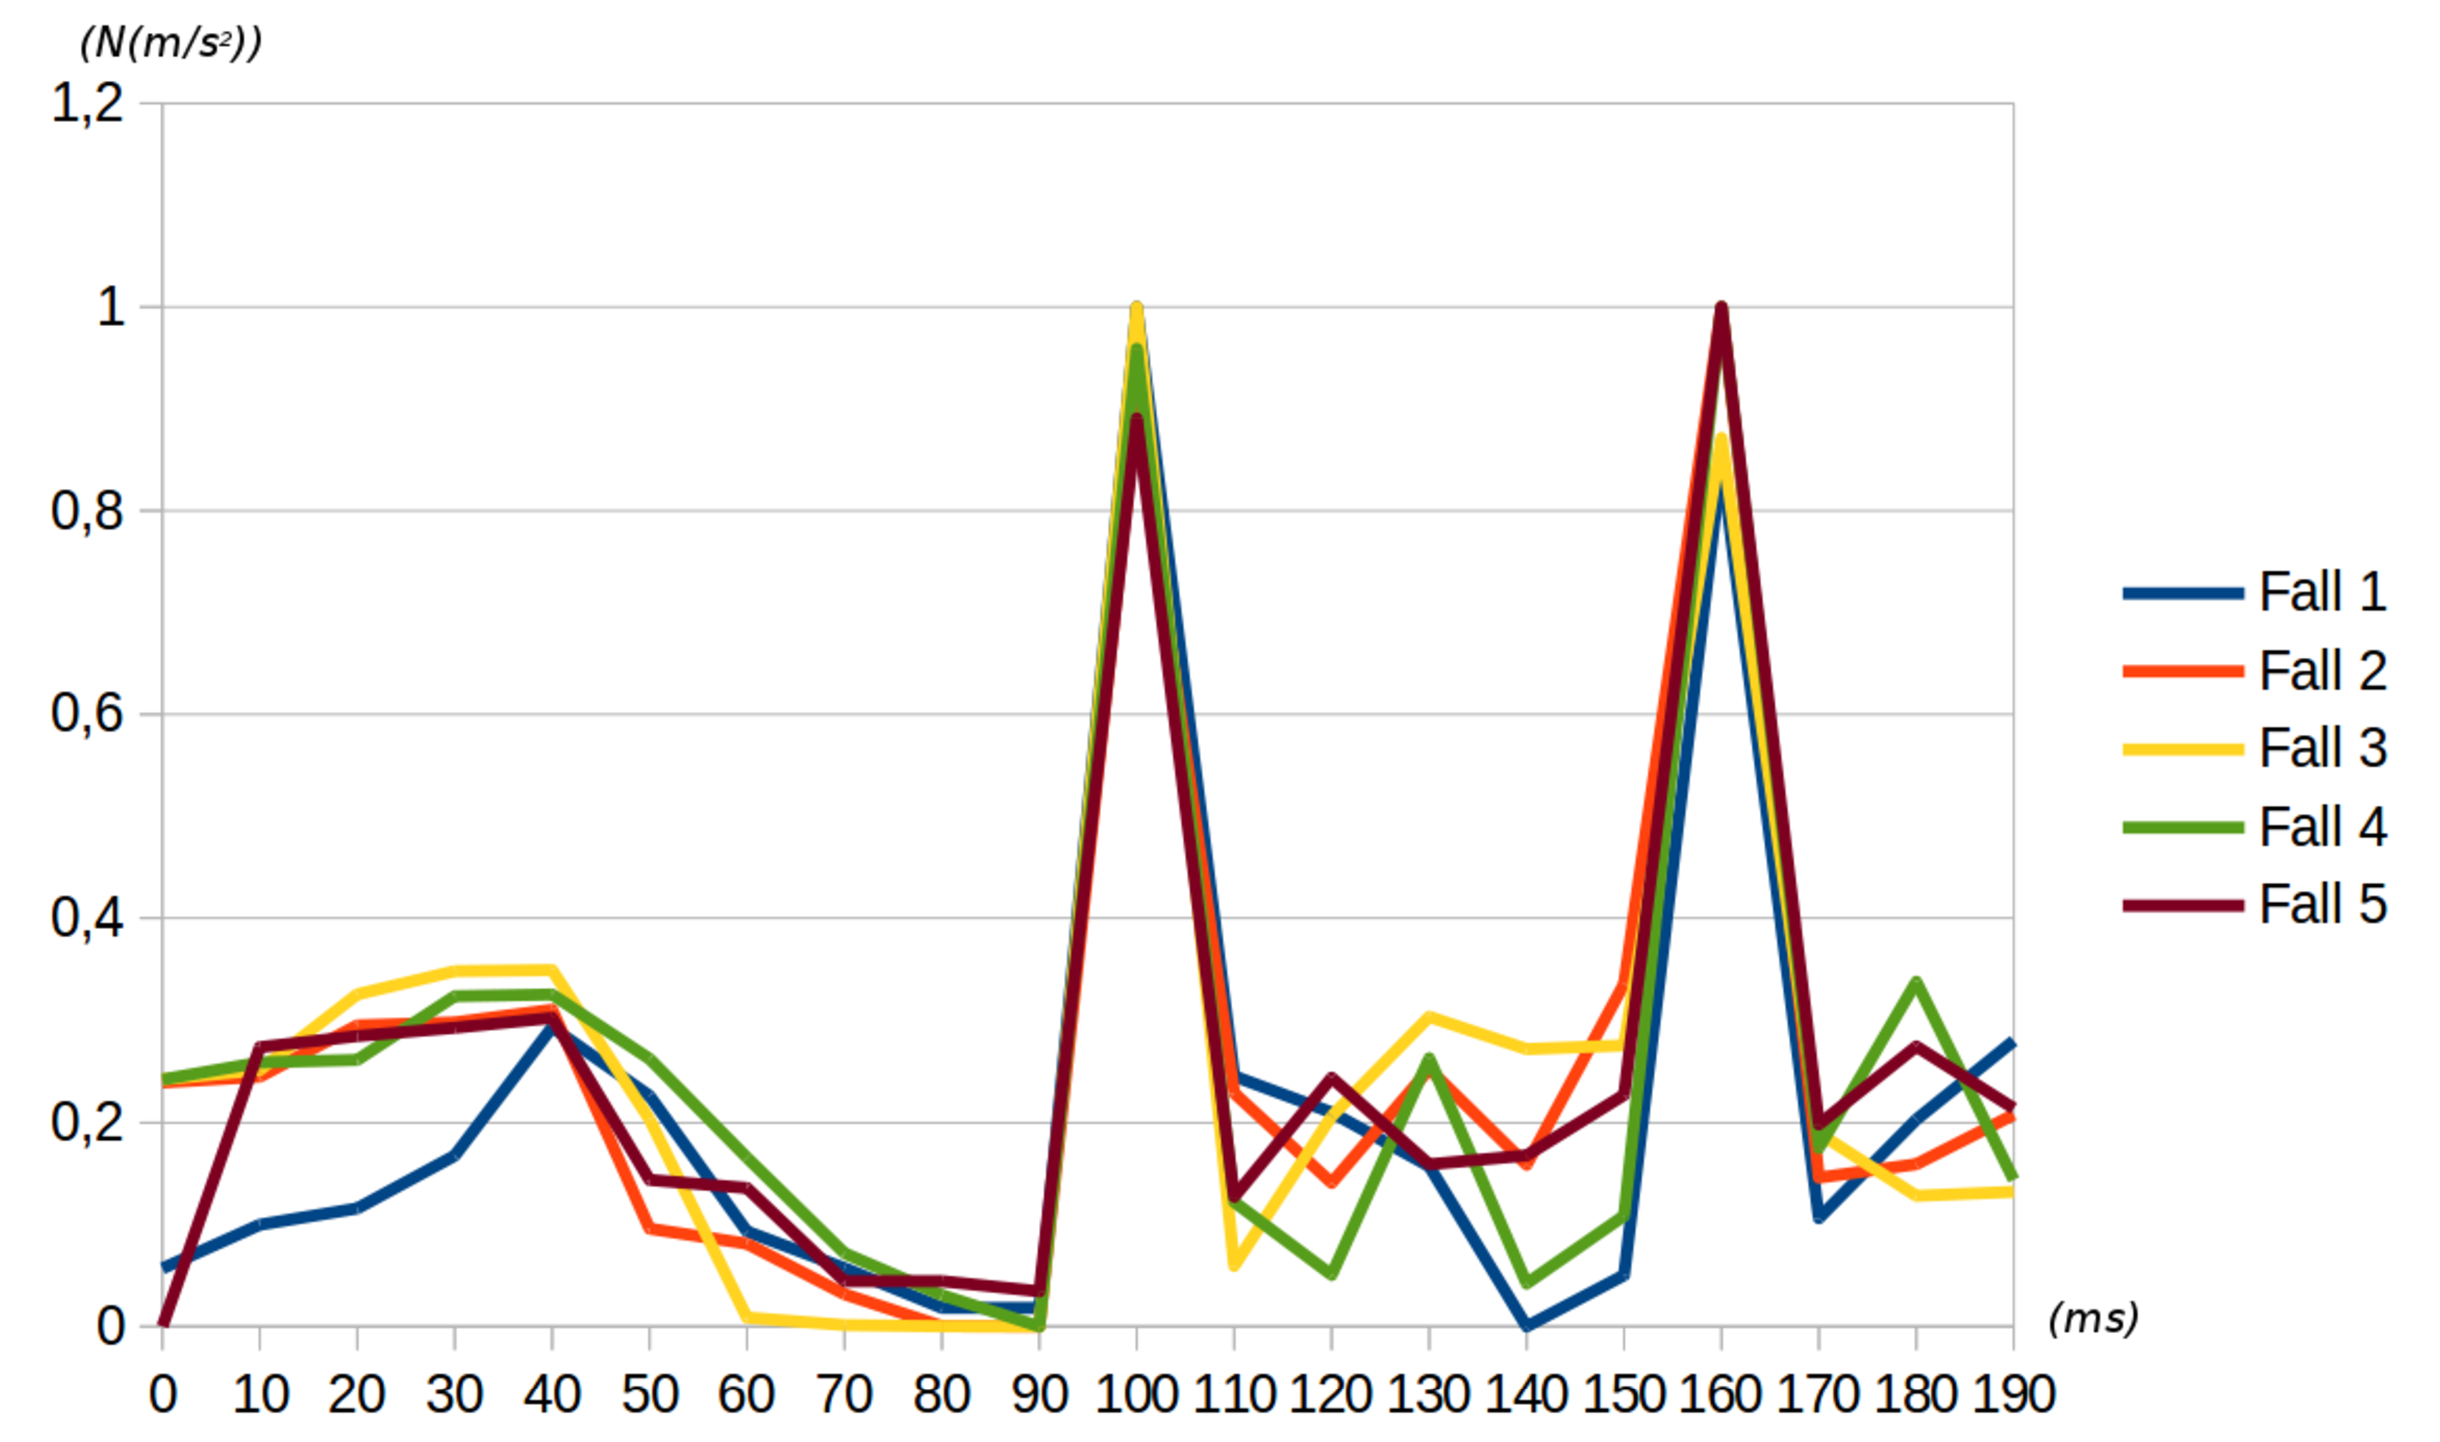
\includegraphics[scale=0.22]{Images/IoTTEGFAWGeneratedEvents.eps}
	\caption[IoT-TEG generated FAW falls]{IoT-TEG generated FAW falls.}
	\label{fig:IoTTEGFAWGeneratedEvents}
\end{figure}

\subsection{Sensor fusion}
\label{subsec:sensorfusion}	
Analyzing the literature regarding fall detection, the existing solutions show certain weaknesses in the reliable detection of falls \cite{Igual2013, Li2009, Luder2009, Pannurat2014, jamsa2014fall}. Considering the approach of Gjoreski et al. \cite{Gjoreski2014}, the results with the fusion of physical sensors and the ECG sensor increase reliability. Especially the evaluation of the ECG signal leads to an essential improvement of the system's accuracy.  According to \cite{Gjoreski2014} the ECG signal could be used to distinguish between different postures. The inclusion of medical parameters could even provide a fall prediction that would represent a significant progress in health care and prevent fatal injuries. Based on these results the proposed fall detection belt has been upgraded with a portable 3-channel ECG sensor. The successive illustration depicts the BAN structure of the update prototype architecture.
\begin{figure}[!ht]
	\centering
	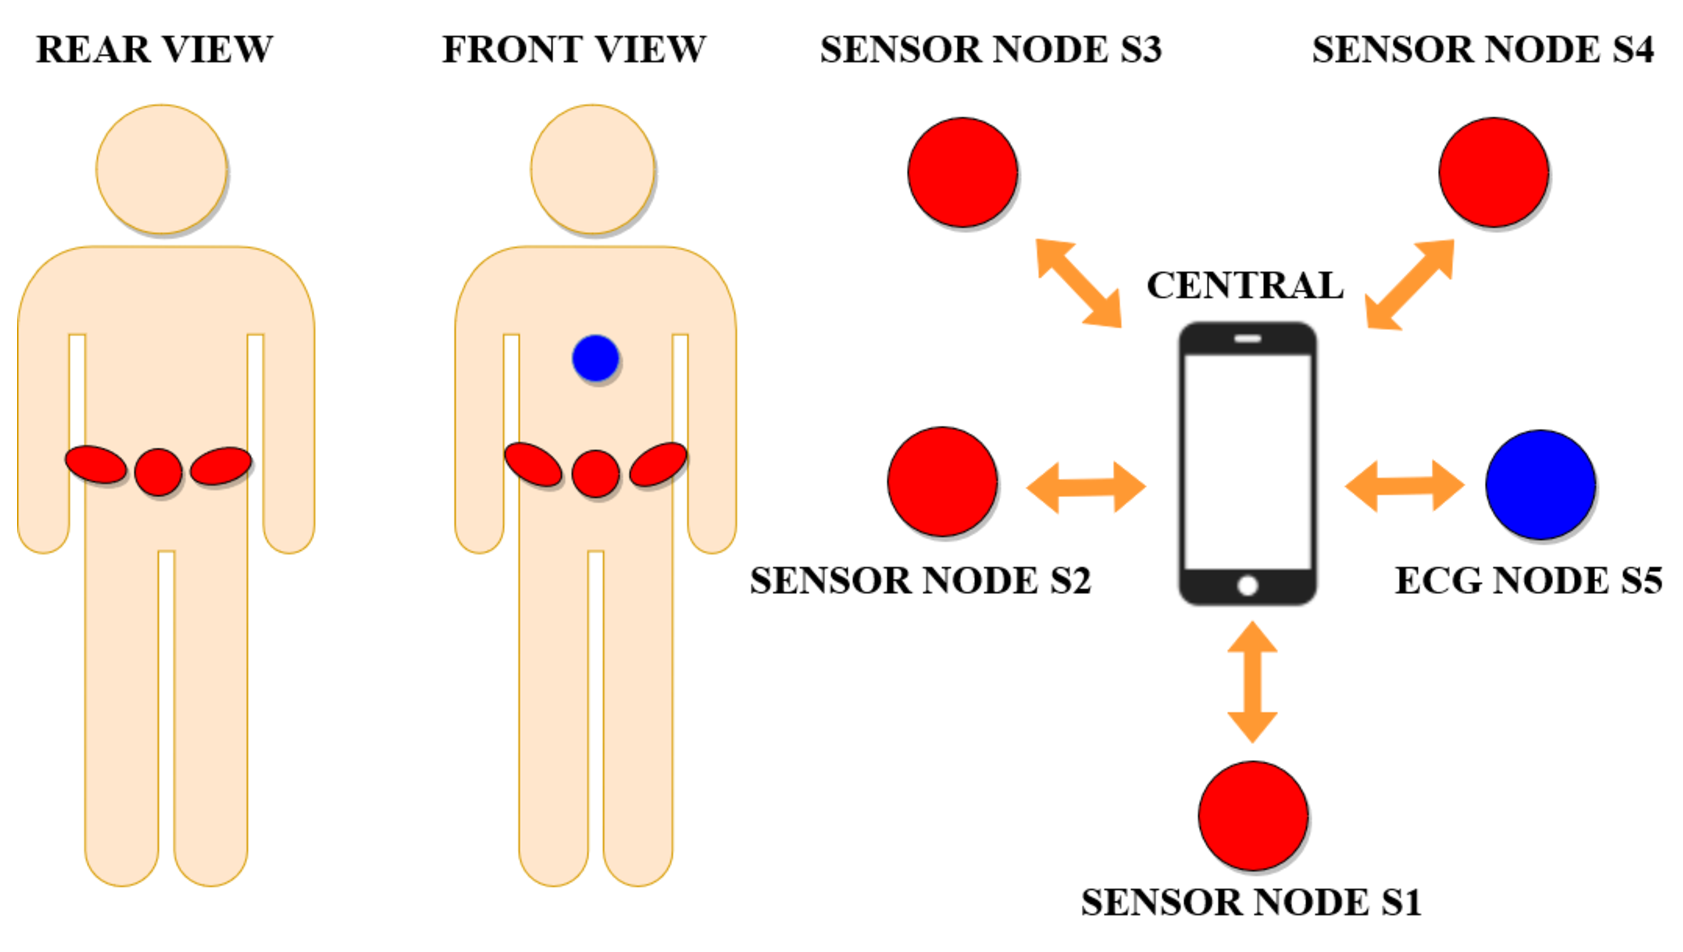
\includegraphics[scale=0.26]{Images/ECG-BAN.eps}
	\caption[ECG BAN]{ECG BAN}
	\label{fig:ECGBAN}
\end{figure}

The updated BAN includes four sensor nodes placed on the belt (S1 - S4) and an additional node on the chest (S5). These five nodes are acting as peripherals and they are continuously providing sensor data to the smartphone (central) via BLE. The sensor nodes S1 to S4 send the acceleration data and the ECG sensor sends ECG signals to the central device. Fusing this information the central device analyzes the events for possible fall events.

Before the ECG sensor can be fully integrated into the prototype, some tasks had be solved. The first task to solve is a continuous recording of the ECG during the person's daily activities. When the ECG electrodes lose contact with the skin surface because of movement, this leads to increased noise in the signal. Therefore, a solution for reliable ECG recording have to be developed. The second task is to perform a validation of the ECG sensor. For this purpose, the  ECG measurements must be compared with measurements taken by a clinical ECG device. Based on Gjoreski et al. \cite{Gjoreski2014} the ECG signal can be relevant to detect fall events as mentioned in Section \ref{sec:relatedwork}. Based on this, another task will be the determination of ECG patterns that provide relevant information for fall events.

The first test measurements with the ECG sensor confirmed the noisy and unstable ECG signal during movements. To ensure a stable and continuous signal during daily activities, an adjustable and flexible ECG harness has been developed with prefabricated electrodes positioning and the ability to adapt to any body shape (see Figure \ref{fig:ECGHarness}).
\begin{figure}[!ht]
	\centering
	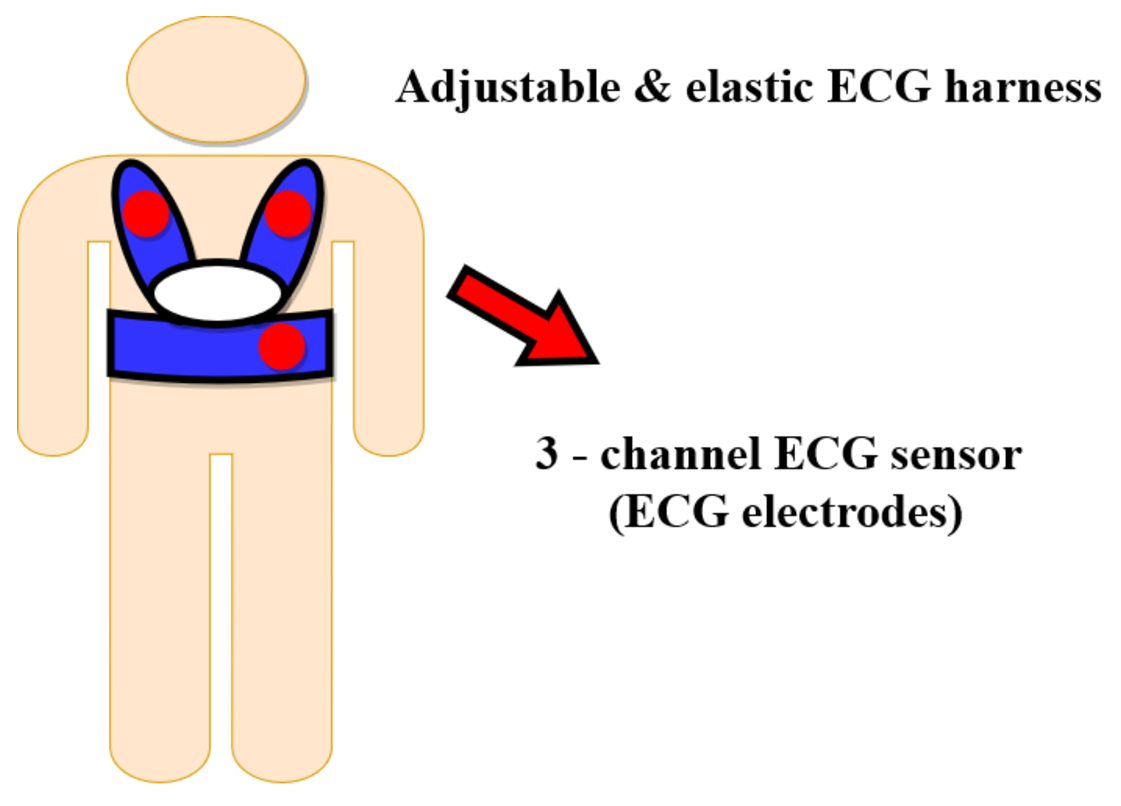
\includegraphics[scale=0.29]{Images/ECG-Harness.eps}
	\caption[ECG - Harness]{ECG harness}
	\label{fig:ECGHarness}
\end{figure}

After completing the development of the ECG harness the measurements were repeated using the harness solution. A more stable signal resulted, especially during walking and the sitting procedure the stability of the ECG signal was improved significantly. The artifacts in an ECG signal which result during motion may be used as a recognition pattern for fall events. After the positive results regarding the improvements of the signal's stability, validation tests were conducted in a medical lab with the assistance of a physician. In clinical settings ECG devices with 10 electrodes are being used but for wearable or emergency purposes (e.g. ambulance) a 3-Channel ECG device is recommended because it provides less wiring and satisfies the aspect of patient compliance \cite{DrNicoletteWagner}. According to a study by Antonicelli et al. \cite{Antonicelli-ECG}, the use of a 3-lead ECG may be essential to avoid delayed treatment of specific heart diseases, such as elderly people who suffer from chronic heart disease and need continuous ECG monitoring. In addition, the analysis in \cite{Antonicelli-ECG} led to the result that a 3-lead ECG provides qualitatively similar evaluation as a 12-lead ECG. Comparing the measurements taken in the medical lab with the ECG measurements provided by our ECG sensor the correct functionality of our sensor could be confirmed. Based on this state of knowledge, ECG measurements are performed during the fall simulations based on \cite{Li2009} and \cite{Pannurat2014} as part of a master thesis \cite{FatimaMasterThesis}. The aim of this work has been to evaluate the ECG patterns for essential artifacts during the fall and to apply machine learning methods to improve the system's ability to detect fall events and, if possible, predict fall events with the additional information of the ECG sensor. The application of machine learning techniques based on accelerometer data is also being investigated. 

\subsection{Detected problems}
\label{sub:detectedproblems}

After testing the used fall detection prototype, some problems were 
found. Moreover, some considerations will be applied in future tests.

First of all, we are going to explain the problems related to the current prototype. The synchronization in the prototype is an issue. There is a lack of synchronization not only in the amount of data, but also in the timestamp. Some sensors transmit more data than the others. The four sensors were working during the FAW fall test, but the obtained acceleration values were from three of them, one of the sensors did not transmit data in one period of the test. 

A hardware issue is the durability of the battery, which is 2 to 3 weeks depending on the use. If we want to use this system in everyday life, we have to make sure that the battery life is extended. If we consider the used ECG sensor architecture, we encountered differences in signal quality that includes noise and baseline shifting (see Figure \ref{fig:ECGBaselineShifting}). 
\begin{figure}[!ht]
	\centering
	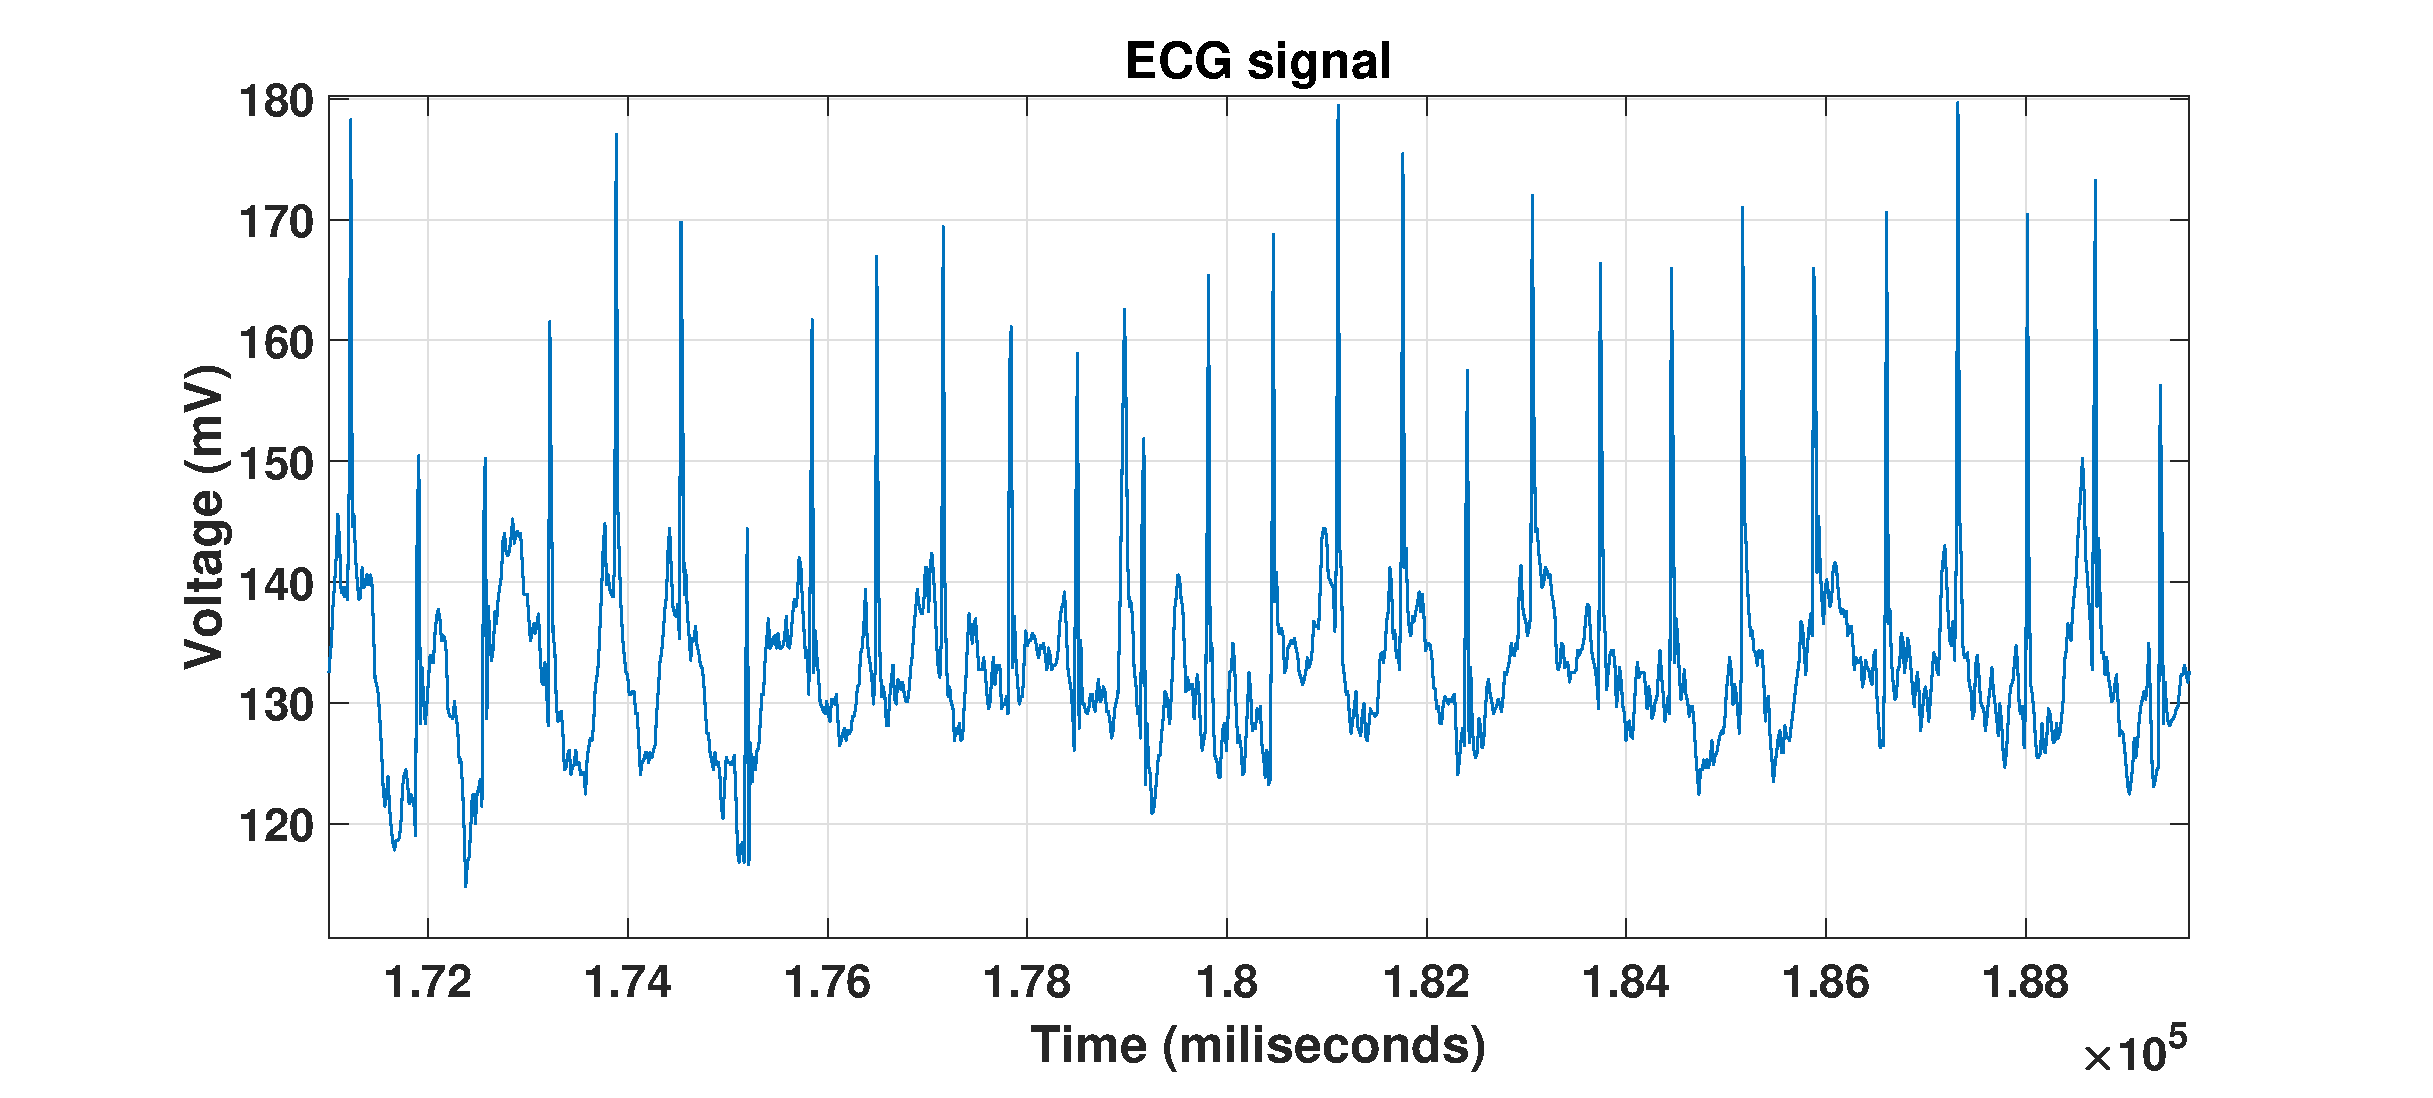
\includegraphics[scale=0.2425]{Images/NormalECG1.eps}
	\caption[Measured ECG signal]{Baseline shifting ECG signal \cite{FatimaMasterThesis}}
	\label{fig:ECGBaselineShifting}
\end{figure}

The reasons for these distinctions in signal quality were explained by the supervising physician. Baseline wander (BW) disturbances are caused by variations in electrode-skin impedance, patient's movement and breathing during the ECG measurements. Muscle contraction is common for people which suffer from tremor or fearing the ECG measurement and for disabled people. Certified clinical devices have an integrated filter which can be applied to smooth the signal \cite{ECGNoise,DrNicoletteWagner}. To solve this problem the application of a low and high pass filter in our setup is considered \cite{FatimaMasterThesis}.

Regarding the analysis of the acceleration values, it was observed that some values could lead to misinterpretation. The reason was that the test persons quickly got up after the fall simulation instead of lying on the ground.
Since not only the measured values but also the video recordings of the fall simulations were analyzed for a profound analysis, the problem could be determined. In a real situation, if a person falls and is able to stand up quickly it means that the person is conscious and able to move. On the contrary, if the person falls and does not get up after a while, it means that the person may be unconscious or unable to make the emergency call.  Therefore, waiting at least 10 seconds in our test scenarios is helpful to perform an accurate fall analysis during testing.

\section{Example application of STAMP as hazard analysis method}
\label{sec:STAMP}

\subsection{Introducing STAMP}
A fall detection system is a safety critical system requiring certification according to a safety standard (e.g. IEC 60601-1-11) \cite{international2005medical}. To satisfy functional safety requirements it is fundamental to apply hazard analysis methods during all development phases and operation to analyze the behavior of the system in case of malfunctioning \cite{STAMPThesis}. In the following STAMP will be applied in some architectural parts of the fall detection system for functional safety validation.

STAMP is a comprehensive hazard analysis method based on system theory. A major goal of this approach is to control or eliminate hazards. This approach proposed by Leveson \cite{leveson2011engineering} is used to identify probable accident causes that are categorized as follows:
\begin{itemize}
	\item Accidents based on hardware and software component failure
	\item Unsafe interactions among components
	\item Complex human machine interfaces and human error models
	\item Erros in system design
	\item Faulty requirements
\end{itemize}  
STAMP treats accidents as a control problem. To prevent accidents safety constraints derived from system safety requirements must be enforced inside the different system hierarchy levels. If the given safety constraints are violated accidents may occur. Checking the enforcement of safety constraints leads to an additional layer of system testing. 

\subsection{STAMP - Hazard analysis}
STAMP begins on the system level and proceeds top down into the system hierarchy. The hierarchical-based analysis in STAMP is based on control loop structures which are iterated from the high abstract level (overall system view) to the lower system levels to build up hierarchical system models \cite{leveson2011engineering}. 
The controller unit of the control structure is acting as a master and includes a process model to determine control actions that are executed by the actuators to control the defined process (controlled process). A feedback loop (measured variables) is provided by the sensor unit which informs the controller about the process state. This information is used by the master to initiate a control action (controlled variables) to run the system within predefined limits. 

STAMP procedures:

\begin{itemize}
	\item \textbf{Definition of accidents:} Person has fallen and the fall was not detected by the system.
	\item \textbf{Definition of hazards:} Data from 1 to 4 sensors of the belt are not sufficiently correlated in time (synchronization error).
	\item \textbf{Definition of safety requirements and constraints:} The safety requirements and constraints are based on the hazard which causes the accident. Safety constraints are used to describe non-permissible system operations in order to ensure safe operating conditions. A top level safety requirement is the real time detection of fall events. The timestamps of all four nodes must be synchronized. If constraints are violated system migrates to unsafe or hazardous state.
	\item \textbf{Definition of safety control structure:}
	A high-level safety control structure should be defined which contains the system's components and the process which should be controlled. The control structure below (see Figure. \ref{fig:STAMPLevel1}) depicts the control loop of the controlled process, the movement of the person.
	The sensors provide sensor data to the controller (smartphone application). The smartphone contains a data acquisition algorithm to collect the incoming data and a fall detection algorithm to analyze this data. If the event corresponds to a fall, the alert system on the mobile device will call the emergency services for intervention. The actuator part of the system contains the control of the data acquisition process, i.e. timers, sleep mode etc.
\end{itemize}	
	The lower level control loops (see Figures \ref{fig:STAMPLevel2+3} and \ref{fig:STAMPLevel4+5}) illustrate a detailed internal control structure of the controlled processes. These processes are interacting as a controller in the lower level structures. Taking into consideration the second level safety control loop, the movement process control (controller) receives the sensor data. Based on the data a control command will be executed to control the BAN which sends a feedback to the movement process controller. The third level control loop zooms into the BAN control, which is the master (controller) that actuates the wake up procedure of the sensor nodes to control the nodes. These will deliver sensor data, including the time to the BAN control.
	\begin{figure}[!ht]
		\centering
		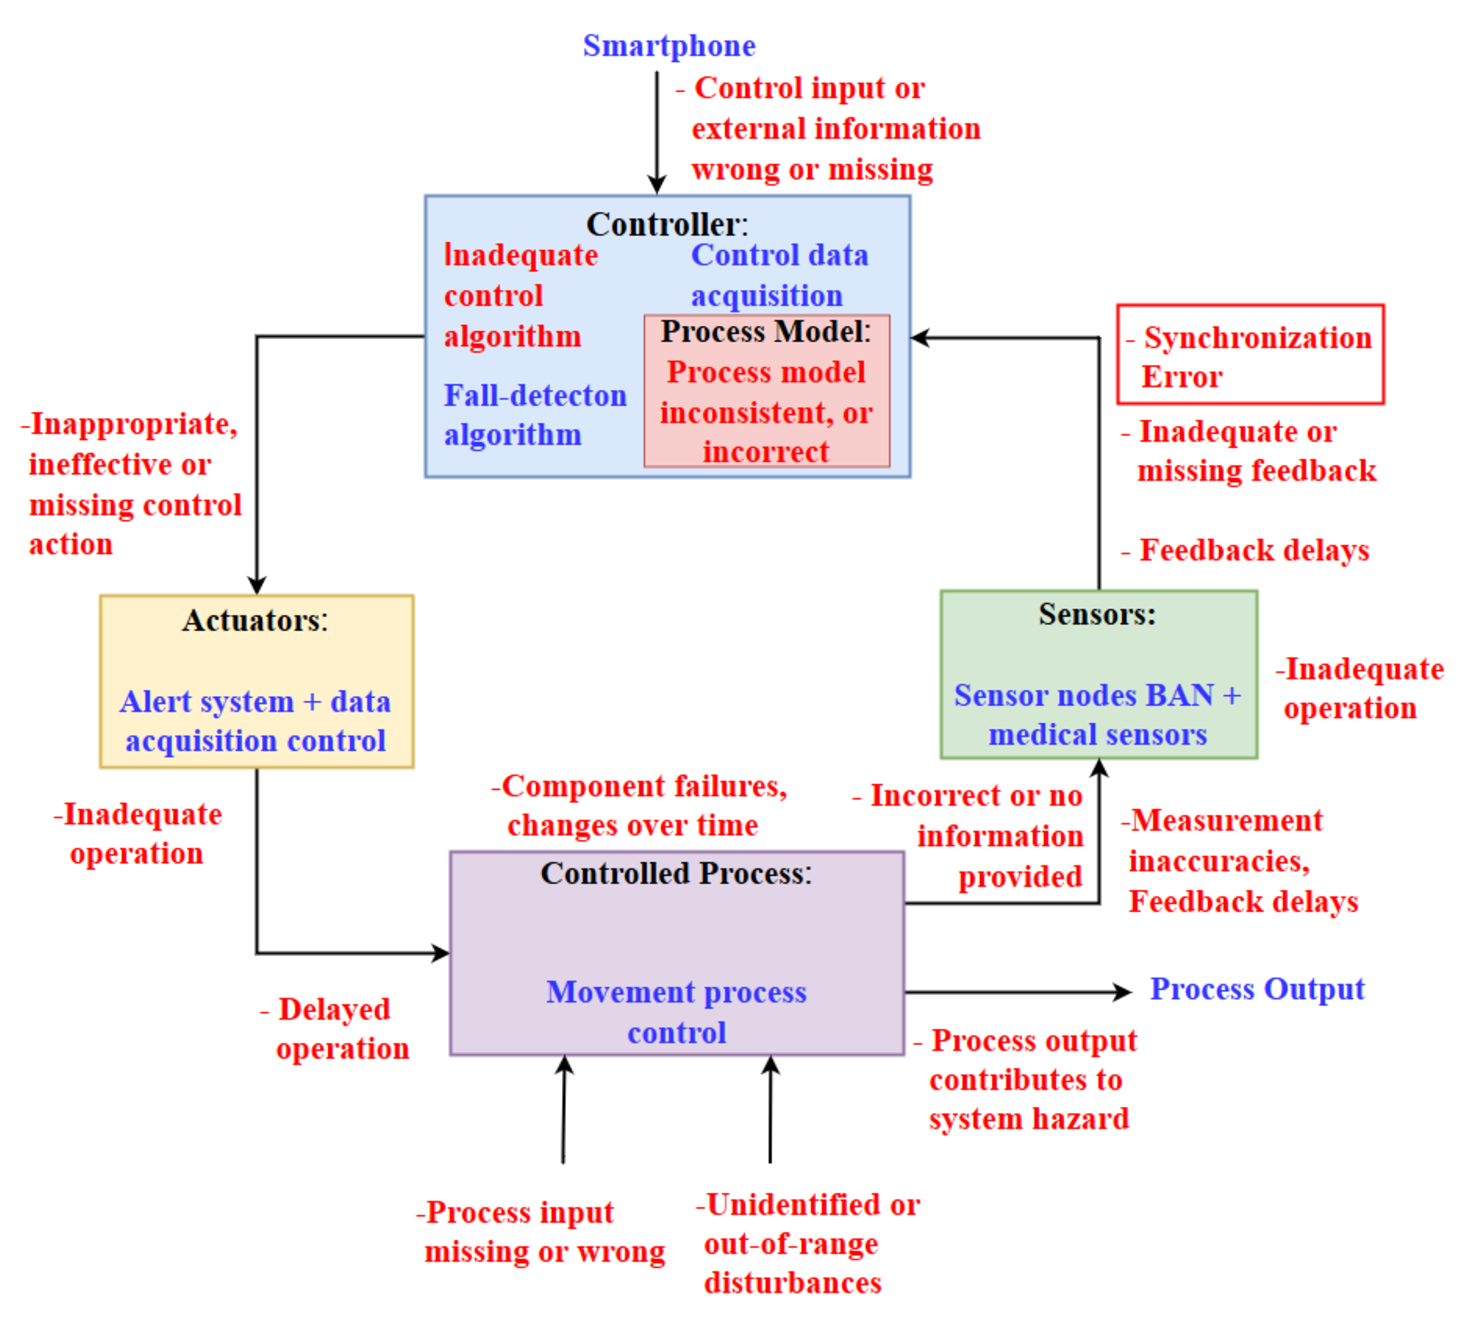
\includegraphics[scale=0.3725]{Images/STAMP_SynchError.eps}
		\caption[System Safety Control Structure]{System Safety Control Structure - Hierarchy level 1) $\rightarrow$ Black label (system components), \textcolor{blue}{blue label (description of system components)}, \textcolor{red}{red label (possible hazards)}}
		\label{fig:STAMPLevel1}
	\end{figure}

	The lower level control loops (see Figures \ref{fig:STAMPLevel2+3} and \ref{fig:STAMPLevel4+5}) illustrate a detailed internal control structure of the controlled processes. These processes are interacting as a controller in the lower level structures. Taking into consideration the second level safety control loop, the movement process control (controller) receives the sensor data. Based on the data a control command will be executed to control the BAN which sends a feedback to the movement process controller. The third level control loop zooms into the BAN control, which is the master (controller) that actuates the wake up procedure of the sensor nodes to control the nodes. These will deliver sensor data, including the time to the BAN control.
	\begin{figure}[!ht]
		\centering
		\includegraphics[scale=0.37]{Images/STAMP2+3level(3).eps}
		\caption[Safety Control Structure - Hierarchy level 2 \& 3]{Safety Control Structure - Hierarchy level 2 \& 3}
		\label{fig:STAMPLevel2+3}
	\end{figure} 

	To provide a more detailed hazard analysis two more control loop layers were created which are illustrated in the successive illustration (see Figure  \ref{fig:STAMPLevel4+5}). The fourth level of the system's control structure zooms into Sensor node control (controlled process in Figure \ref{fig:STAMPLevel2+3}) which is the control unit (controller). Considering this control layer the controller receives the sensor's services and characteristics which are provided via BLE and contain the sensor values. The sensor node control initiates a scanning command (actuator) to detect the sensor properties which are provided by the BLE interface (controlled process: Bluetooth sensor detection control).  
	
	\begin{figure}[!ht]
		\centering
		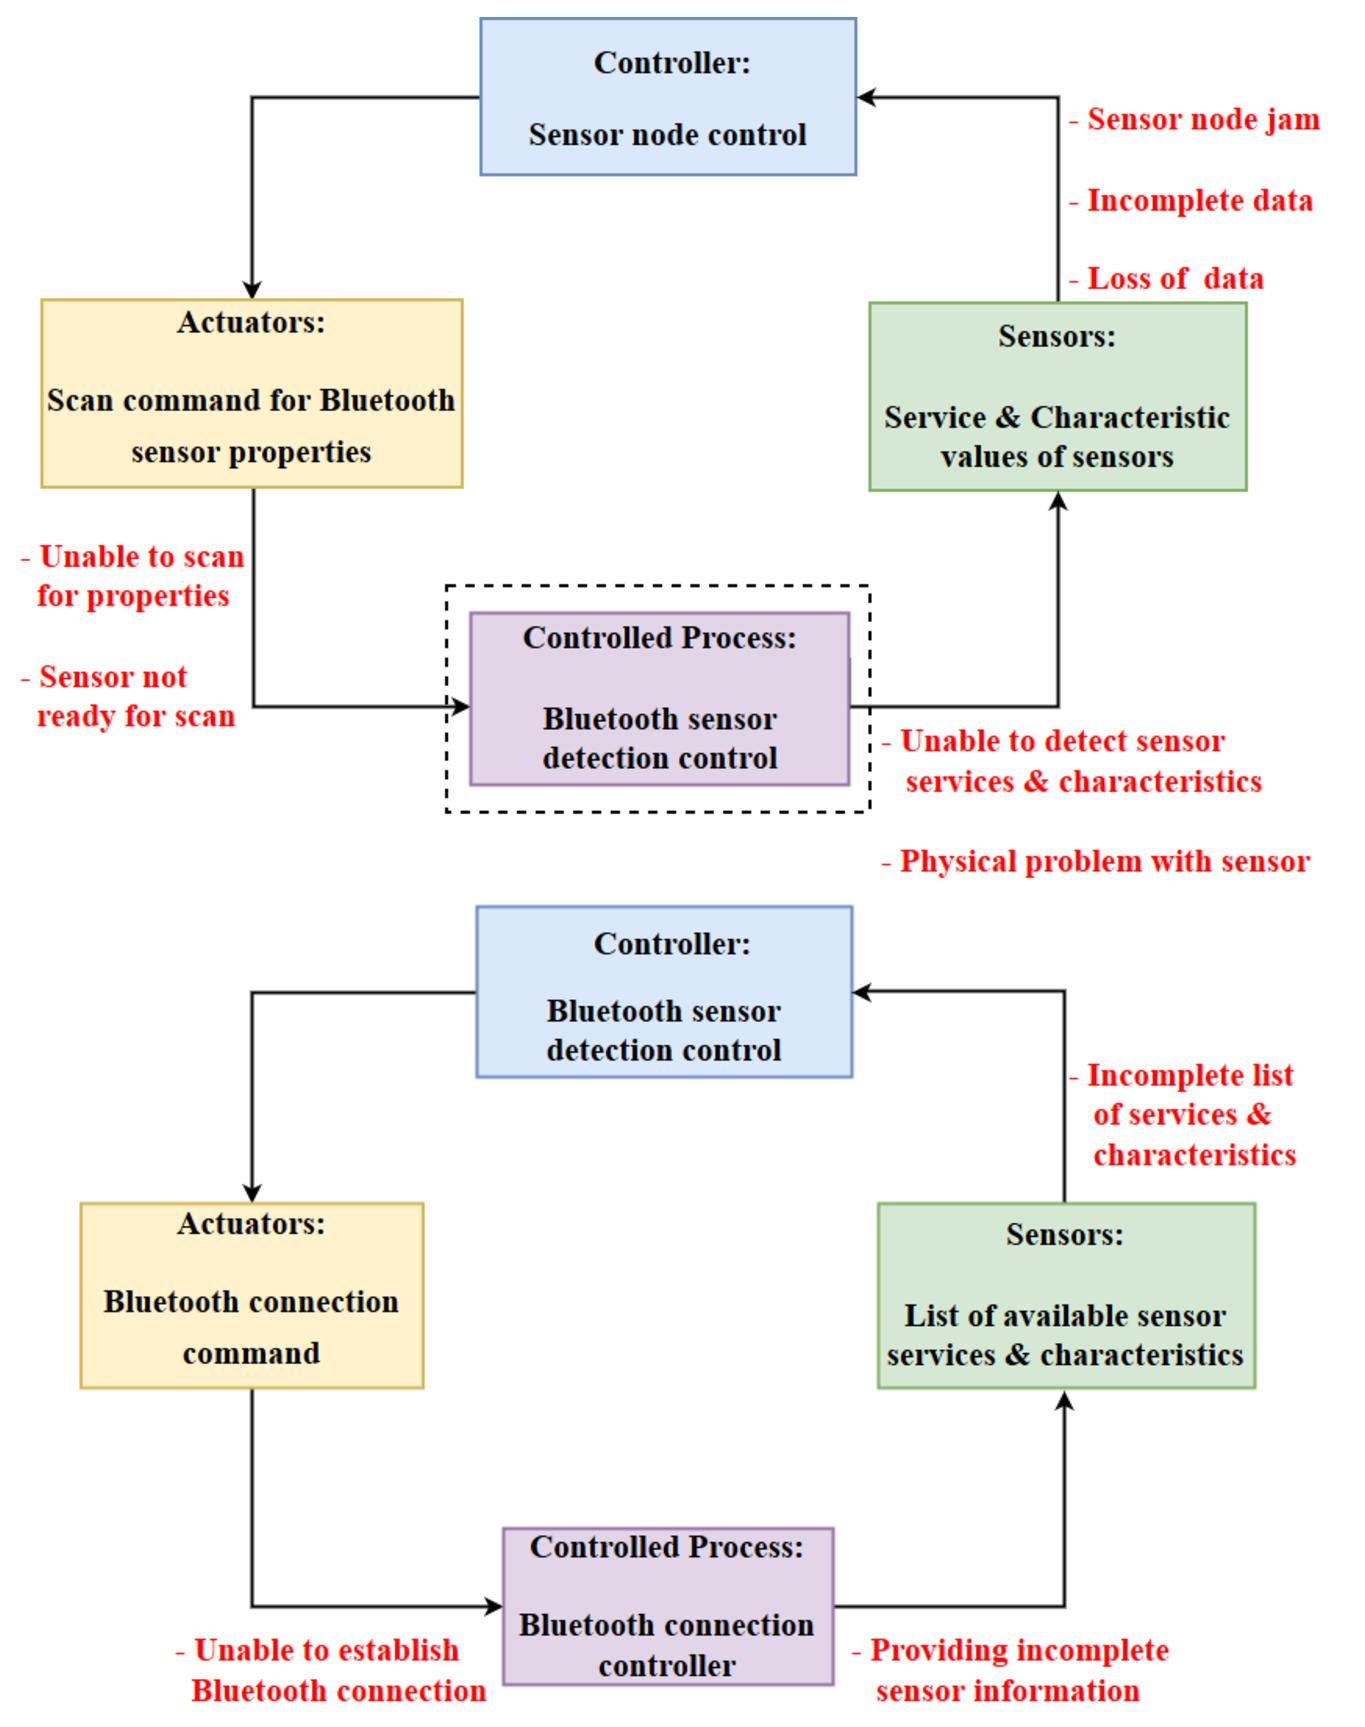
\includegraphics[scale=0.3675]{Images/STAMP4+5level(2).eps}
		\caption[Safety Control Structure - Hierarchy level 4 \& 5]{Safety Control Structure - Hierarchy level 4 \& 5}
		\label{fig:STAMPLevel4+5}
	\end{figure}
	
	Taking into consideration the fifth level of the control loop which is depicted in Figure \ref{fig:STAMPLevel4+5} an accurate view of the controlled process Bluetooth sensor detection control in level 4 is provided. The master Bluetooth sensor detection control (controller) actuates a connection command via BLE (actuator) to establish a connection to the sensors (controlled process: Bluetooth connection control) which sends a list of available sensor's services and characteristics to the controller. 
	
	All these hazards (see red labels in Figure \ref{fig:STAMPLevel1}, \ref{fig:STAMPLevel2+3}, \ref{fig:STAMPLevel4+5}) lead to safety constraints.
	Some of the safety constraints are defined as follows when considering the control loop structures of the second and third system levels:
	\begin{itemize}
		\item Second level control structure $\rightarrow$ to avoid data loss and provide a reliable evaluation of events by the movement process controller, the sensors should provide synchronized data.
		\item Third level control structure $\rightarrow$ a synchronous wake up procedure of all sensors in the BAN must be ensured to avoid data loss.
	\end{itemize}
	If the control structures of the fourth and fifth system levels are considered, some of the safety constraints are defined as follows:
	\begin{itemize}
		\item Fourth level control structure $\rightarrow$ It must be ensured that the sensor information (services \& characteristics) is transmitted completely.
		\item Fifth level control structure $\rightarrow$ A reliable and stable BLE connection to all nodes of the BAN must be established.
	\end{itemize}
	Violating one of the above-mentioned safety constraints, a chain reaction of hazards (non-permissible operations) is triggered in all system layers, which leads to malfunction of the system.  The following scenario, which reflects a possible chain reaction of hazards, shows the possible effects on the system functionality.
	The incomplete list of sensor's services and characteristics (control loop - lower level 5) and sensor node jam (control loop - lower level 4) can lead to clock drift (control loop - lower level 3) and unsynchronized data (control loop - lower level 2) in the upper levels. Merging all the hazards from the lower levels may cause the synchronization error (see description in subsection \ref{sub:detectedproblems}) in the top level control structure (see Figure \ref{fig:STAMPLevel1}) and lead to violation of the safety constraint $\Delta$t $<=$ 50ms between the timestamps of the sensor nodes. The combination of these possible hazards makes the system inoperable to detect falls in real time.
	
%\end{itemize}
It is important to emphasize that this is only the beginning of a complete STAMP analysis, which represents a fraction of the system.  We will use it for all parts of the complete architecture.

\section{Findings with respect to the research questions}
\label{sec:FindingsResearchQuestions}
Our ongoing research solved part of the research questions (see Section \ref{sec:introduction}). The following subsections relate our results to the corresponding research questions.

\subsection{Will the integration of medical sensors improve the reliability of the fall detection system?}
\label{subsec:integrationMedicalSensors}
Considering the reliability in relation to the integration of medical sensors in our fall detection system, by analyzing the literature \cite{Gjoreski2014} it can be concluded that medical parameters significantly enhance the capabilities of the fall detection. Consultation with physicians \cite{DrNicoletteWagner} confirmed that the data acquisition of medical parameters in parallel to the acceleration data cover a fall event initiated by medical conditions comprehensively. Our ongoing tests performed with the ECG sensor harness indicate that the ECG provides relevant information for an accurate fall detection. Current work analyzes disturbances of the ECG signal and explores the use of machine learning methods to detect relevant normal and abnormal medical patterns \cite{FatimaMasterThesis}. 

\subsection{Can the system achieve a high level of acceptance among people?}
\label{subsec:acceptanceSystem}
According to the feedback from our test subjects, our system has achieved a high level of acceptance:
\begin{itemize}
	\item The hardware architecture is flexible and adaptable to any body shape.
	\item The current prototype has decreased in size.
	\item With the belt and harness solution, the system is not visible from the outside and can be worn comfortably. This aspect increases patient compliance.
\end{itemize}

\section{Conclusion}
\label{sec:conclusion}
%This work presents a wearable solution for fall detection that enhances the benefits of smart cities in terms of e-health. The growing population and the urban lifestyle require a smart health care system which is capable to provide a fast and efficient medical care. Thinking about the benefits that e-health brings to smart cities, it becomes clear that minimal response times and rapid intervention in emergency situations can significantly improve the population's lives. A typical use case is a smart factory that uses fully automated processes that cause the deployment of a small number of personnel and therefore the workers usually have to work alone in hazardous working conditions. In the case of a fall-event during the night shift, the integration of the portable fall-detection system (e-health) into the smart city infrastructure can provide immediate intervention. 
%
%The tests performed with the test persons provided positive feedback regarding the use of this solution and a high acceptance of the system in conjunction with smart city lifestyle was achieved. These results also show that falls are a general problem in our daily life, which are underestimated and can lead to serious injuries or even fatal consequences. 

This proposed portable fall detection system aims to provide rapid and efficient assistance to people who are in life-threatening situations due to falls. 

The test measurements performed with the test subjects resulted positively regarding the detection of fall events and the acceptance of wearing such a system. Incorporating the ECG sensor proved the effectiveness of Gjoreski et al's concept \cite{Gjoreski2014} combining physical and medical sensor information (acceleration values \& ECG) to ensure more accurate detection of falls and, if necessary, fall prediction. 

Using the IoT-TEG tool \cite{Gutierrez2017,TesisGutierrez2017} facilitates the generation of events to recognize falls which are based on \cite{Kozina}. We have the ability to assign behavior rules to as many event attributes as the event type contains, and the event attribute values follow the specified behavior. IoT-TEG \cite{Gutierrez2017,TesisGutierrez2017} has the ability to adapt the behavior of the analyzed event attribute, because it was designed to generate events of any event type to test systems which manage events. In the further development process it is planned to use machine learning and complementary CEP in order to use certain ECG patterns in combination with the acceleration data. These should enhance a reliable detection of falls. Since the IoT-TEG tool \cite{Gutierrez2017,TesisGutierrez2017} is in constant development to ensure an accurate generation of events, further functionalities will be integrated in the future to meet all test requirements.

However, first the synchronization problem of the BAN must be solved, which can compromise the system's functionality. A new hardware platform will be used, which contains a real time operating system, which facilitates the synchronization of different tasks in a wireless sensor network. In addition, the new microcontroller should also meet other requirements of patient compliance.

Referring to the research questions (see Section \ref{sec:introduction}), several aspects have been solved (see Section \ref{sec:FindingsResearchQuestions}). Due to the complex nature of the problem, ongoing research is being done to enhance the quality of the solution.

\section*{Acknowledgments}
We would like to thank the voluntary test subjects for the time they spent testing the fall detection prototype. The feedback and test results are very valuable for the further development of the detection system. We would particularly like to thank Dr. med. Nicolette Fritsch-Wagner for her assistance during the validation of our ECG sensor and for medical advice on ECG analysis. 

Paper partially funded by The Ministry of Economy and Competitiveness (Spain) and the FEDER Fund, under the National Program for Research, Development and Innovation, Societal Challenges Oriented, Project DArDOS TIN2015-65845-C3-3-R and Project FAME (RTI2018-093608-B-C33).


% An example of a floating figure using the graphicx package.
% Note that \label must occur AFTER (or within) \caption.
% For figures, \caption should occur after the \includegraphics.
% Note that IEEEtran v1.7 and later has special internal code that
% is designed to preserve the operation of \label within \caption
% even when the captionsoff option is in effect. However, because
% of issues like this, it may be the safest practice to put all your
% \label just after \caption rather than within \caption{}.
%
% Reminder: the "draftcls" or "draftclsnofoot", not "draft", class
% option should be used if it is desired that the figures are to be
% displayed while in draft mode.
%
%\begin{figure}[!t]
%\centering
%\includegraphics[width=2.5in]{myfigure}
% where an .eps filename suffix will be assumed under latex, 
% and a .pdf suffix will be assumed for pdflatex; or what has been declared
% via \DeclareGraphicsExtensions.
%\caption{Simulation results for the network.}
%\label{fig_sim}
%\end{figure}

% Note that the IEEE typically puts floats only at the top, even when this
% results in a large percentage of a column being occupied by floats.
% However, the Computer Society has been known to put floats at the bottom.


% An example of a double column floating figure using two subfigures.
% (The subfig.sty package must be loaded for this to work.)
% The subfigure \label commands are set within each subfloat command,
% and the \label for the overall figure must come after \caption.
% \hfil is used as a separator to get equal spacing.
% Watch out that the combined width of all the subfigures on a 
% line do not exceed the text width or a line break will occur.
%
%\begin{figure*}[!t]
%\centering
%\subfloat[Case I]{\includegraphics[width=2.5in]{box}%
%\label{fig_first_case}}
%\hfil
%\subfloat[Case II]{\includegraphics[width=2.5in]{box}%
%\label{fig_second_case}}
%\caption{Simulation results for the network.}
%\label{fig_sim}
%\end{figure*}
%
% Note that often IEEE papers with subfigures do not employ subfigure
% captions (using the optional argument to \subfloat[]), but instead will
% reference/describe all of them (a), (b), etc., within the main caption.
% Be aware that for subfig.sty to generate the (a), (b), etc., subfigure
% labels, the optional argument to \subfloat must be present. If a
% subcaption is not desired, just leave its contents blank,
% e.g., \subfloat[].


% An example of a floating table. Note that, for IEEE style tables, the
% \caption command should come BEFORE the table and, given that table
% captions serve much like titles, are usually capitalized except for words
% such as a, an, and, as, at, but, by, for, in, nor, of, on, or, the, to
% and up, which are usually not capitalized unless they are the first or
% last word of the caption. Table text will default to \footnotesize as
% the IEEE normally uses this smaller font for tables.
% The \label must come after \caption as always.
%
%\begin{table}[!t]
%% increase table row spacing, adjust to taste
%\renewcommand{\arraystretch}{1.3}
% if using array.sty, it might be a good idea to tweak the value of
% \extrarowheight as needed to properly center the text within the cells
%\caption{An Example of a Table}
%\label{table_example}
%\centering
%% Some packages, such as MDW tools, offer better commands for making tables
%% than the plain LaTeX2e tabular which is used here.
%\begin{tabular}{|c||c|}
%\hline
%One & Two\\
%\hline
%Three & Four\\
%\hline
%\end{tabular}
%\end{table}


% Note that the IEEE does not put floats in the very first column
% - or typically anywhere on the first page for that matter. Also,
% in-text middle ("here") positioning is typically not used, but it
% is allowed and encouraged for Computer Society conferences (but
% not Computer Society journals). Most IEEE journals/conferences use
% top floats exclusively. 
% Note that, LaTeX2e, unlike IEEE journals/conferences, places
% footnotes above bottom floats. This can be corrected via the
% \fnbelowfloat command of the stfloats package.




%\section{Conclusion}
%The conclusion goes here.





% if have a single appendix:
%\appendix[Proof of the Zonklar Equations]
% or
%\appendix  % for no appendix heading
% do not use \section anymore after \appendix, only \section*
% is possibly needed

% use appendices with more than one appendix
% then use \section to start each appendix
% you must declare a \section before using any
% \subsection or using \label (\appendices by itself
% starts a section numbered zero.)
%


\appendices
\section{Datasets}
\cite{FallRepo} is a dataset repository which contains: fall simulation data, fall analysis, IoT-TEG generated test events and fall simulation video clip.

% you can choose not to have a title for an appendix
% if you want by leaving the argument blank
%\section{}
%Appendix two text goes here.


%% use section* for acknowledgment
%\ifCLASSOPTIONcompsoc
%  % The Computer Society usually uses the plural form
%  \section*{Acknowledgments}
%\else
%  % regular IEEE prefers the singular form
%  \section*{Acknowledgment}
%\fi
%
%
%The authors would like to thank...


% Can use something like this to put references on a page
% by themselves when using endfloat and the captionsoff option.
\ifCLASSOPTIONcaptionsoff
  \newpage
\fi



% trigger a \newpage just before the given reference
% number - used to balance the columns on the last page
% adjust value as needed - may need to be readjusted if
% the document is modified later
%\IEEEtriggeratref{8}
% The "triggered" command can be changed if desired:
%\IEEEtriggercmd{\enlargethispage{-5in}}

% references section

% can use a bibliography generated by BibTeX as a .bbl file
% BibTeX documentation can be easily obtained at:
% http://mirror.ctan.org/biblio/bibtex/contrib/doc/
% The IEEEtran BibTeX style support page is at:
% http://www.michaelshell.org/tex/ieeetran/bibtex/
%\bibliographystyle{IEEEtran}
% argument is your BibTeX string definitions and bibliography database(s)
%\bibliography{IEEEabrv,../bib/paper}
\bibliographystyle{IEEEtran}
% <OR> manually copy in the resultant .bbl file
% set second argument of \begin to the number of references
% (used to reserve space for the reference number labels box)
%\begin{thebibliography}{1}

%\bibitem{IEEEhowto:kopka}
%H.~Kopka and P.~W. Daly, \emph{A Guide to \LaTeX}, 3rd~ed.\hskip 1em plus
  %0.5em minus 0.4em\relax Harlow, England: Addison-Wesley, 1999.

%\end{thebibliography}
\bibliography{references}
% biography section
% 
% If you have an EPS/PDF photo (graphicx package needed) extra braces are
% needed around the contents of the optional argument to biography to prevent
% the LaTeX parser from getting confused when it sees the complicated
% \includegraphics command within an optional argument. (You could create
% your own custom macro containing the \includegraphics command to make things
% simpler here.)

%\begin{IEEEbiography}[{\includegraphics[width=1in,height=1.25in,clip,keepaspectratio]{mshell}}]{Michael Shell}
% or if you just want to reserve a space for a photo:
\begin{IEEEbiography}[{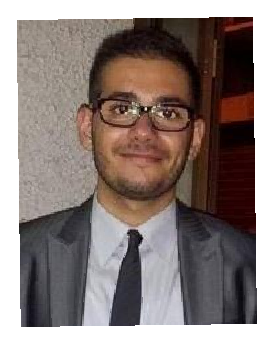
\includegraphics[width=1in,height=1.25in,clip,keepaspectratio]{Images/luigi.eps}}]{Luigi La Blunda}
 received his Bachelor of Engineering degree in Engineering Informatics in 2013 and his Master of Science degree in Barrier-free Systems, with the specialization in Intelligent Systems, in 2016 at the Frankfurt University of Applied Sciences (Germany). He has worked as a tutor in the laboratory experiments of electrical engineering, electronics, and in the lectures of software engineering analysis and design. In 2014 Luigi La Blunda became a research assistant in the WSN \& IOT research group at the Frankfurt University of Applied Sciences (Germany). In addition, he supervises the project lecture Smart Sensor Network Systems in the master programs Barrier-free Systems - Intelligent Systems (BaSys), High Integrity Systems (HIS) and Computer Science. The aim of this course is to develop a running Wireless Smart Sensor Network (WSN) prototype.  His research areas are Internet of Things and Wireless Sensor Networks, with specialization in fall analysis and detection. Since 2016 he is a PhD candidate in the PhD program Engineering Informatics at the University of C\'adiz (Spain).
\end{IEEEbiography}
\vfill
\begin{IEEEbiography}[{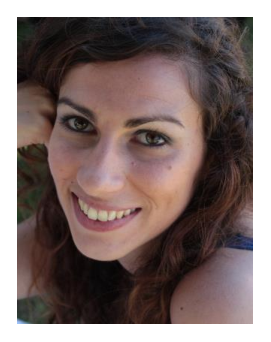
\includegraphics[width=1in,height=1.25in,clip,keepaspectratio]{Images/lorena.eps}}]{Lorena Guti\'errez-Madro\~nal}
	received her first-class Honours Degree in Computer Systems Management in 2007, her BSc in Computer Science in 2009, her Master of Advanced Studies in Computer Science in 2010 and her PhD in 2017 at the University of C\'adiz (Spain). She has been working at the Department of Computer Science and Engineering as a full time lecturer since 2009. Her research is focused on the Internet of Things and test event generation for any event-processing program. In order to prove the usability of the test generated events, she is using them to apply mutation testing to EPL query languages, such as the Event Processing Language (EPL). She has participated in research projects, all involved in software engineering related aspects. She has served in program and organizing committees at different conferences. She is a researcher of the UCASE Software Engineering Research Group. 
\end{IEEEbiography}
\begin{IEEEbiography}[{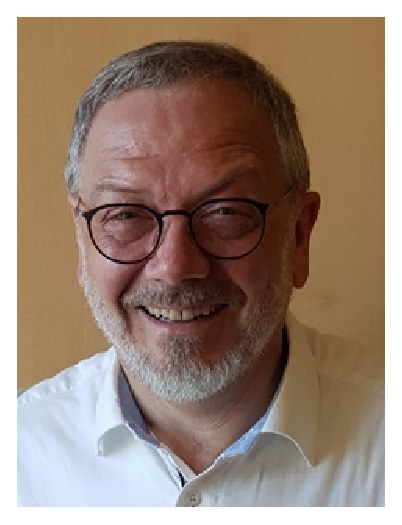
\includegraphics[width=1in,height=1.25in,clip,keepaspectratio]{Images/wagner.eps}}]{Matthias F. Wagner}
	 received a Diploma and a Dr. rer.nat. in Physics from the Johannes Gutenberg - Universität Mainz (Germany). He was Head of Measuring Technology Software Development at Hottinger Baldwin Messtechnik (HBM) in Darmstadt (Germany) from 1990 until 2002. 2002 he was appointed as Professor of Computer Science at the Frankfurt University of Applied Sciences in Frankfurt am Main (Germany). Since 2005 he is Program Director of the international M.Sc. program ``High Integrity Systems''. Since 2017 he is serving as Vice-Dean for Research and International Relations of the FB2, Department of Computer Science and Engineering. Since 2010 he is head of the Research Group Wireless Sensor Networks \& Internet of Things (WSN \& IoT). His research interests cover Safety Critical Computer Systems, Smart Sensor and Actuator Networks, Software and Systems Engineering and Computational Science and is supported by research stays at the UCASE Software Engineering Research Group of the Universidad de C\'adiz (Spain) and the Dipartimento di Fisica e Astronomia of the Università degli Studi di Firenze (Italy). 
\end{IEEEbiography}
\begin{IEEEbiography}[{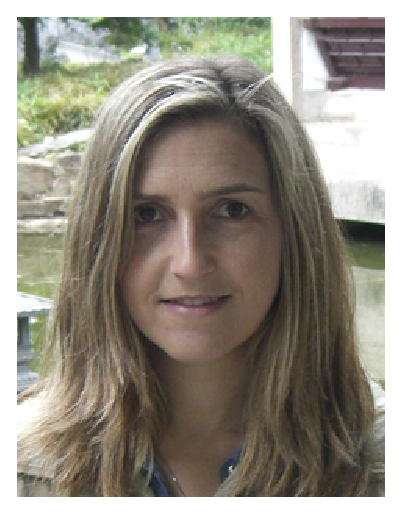
\includegraphics[width=1in,height=1.25in,clip,keepaspectratio]{Images/inma.eps}}]{Inmaculada Medina-Bulo}
	  received her PhD in Computer Science at the University of Seville (Spain). She has been an Associate Professor in the Department of Computer Science and Engineering of the University of C\'adiz (Spain) since 1999. She has been a member of the Council of the School of Engineering (ESI) as well as a Socrates/Erasmus Program Coordinator for several years. From July 2010 to July 2011 she was appointed Degree Coordinator for the Computer Science Studies and a member of the Board of the ESI. Since September 2013 she hold the post of Chief Information Officer of the University. Her research was supported by research stays at the USA, the UK and Germany. She has served in program or organizing committees at different conferences and journals. She has published numerous papers in international journals, and international conference and workshop proceedings. She is the main researcher of the UCASE Software Engineering Research Group. Her main research interests are software verification, software testing, web service compositions, model-driven engineering and complex event processing. She has coordinated the development of several open source testing tools, such as the MuBPEL mutation testing tool for WS-BPEL, the GAmeraHOM tool for locating ``hard-to-kill'' mutants, the Rodan test case generation tool and the Takuan dynamic invariant generator for WS-BPEL. She has participated in and leaded research projects, all involved in software engineering related aspects. 
\end{IEEEbiography}
%\vfill  %---> Adter paragraph (platziert biography weiter oben, näher zur vorgerigen)

% if you will not have a photo at all:
%\begin{IEEEbiographynophoto}{John Doe}
%Biography text here.
%\end{IEEEbiographynophoto}

% insert where needed to balance the two columns on the last page with
% biographies
%\newpage

%\begin{IEEEbiographynophoto}{Jane Doe}
%Biography text here.
%\end{IEEEbiographynophoto}

% You can push biographies down or up by placing
% a \vfill before or after them. The appropriate
% use of \vfill depends on what kind of text is
% on the last page and whether or not the columns
% are being equalized.

%\vfill

% Can be used to pull up biographies so that the bottom of the last one
% is flush with the other column.
%\enlargethispage{-5in}



% that's all folks
\end{document}


